\documentclass[a4paper]{article}
\usepackage[utf8]{inputenc}
\usepackage[russian]{babel}
\usepackage[T2]{fontenc}
\usepackage[warn]{mathtext}
\usepackage{graphicx}
\usepackage{amsmath}
\usepackage{floatflt}
\usepackage{amssymb}
\usepackage[left=20mm, top=20mm, right=20mm, bottom=20mm, footskip=10mm]{geometry}


\graphicspath{ {images/} }
\usepackage{multicol}
\setlength{\columnsep}{2cm}


\begin{document}

\begin{titlepage}
	\centering
	\vspace{5cm}
	{\scshape\LARGE Московский физико-технический институт \par}
	\vspace{4cm}
	{\scshape\Large Лабораторная работа \par}
	\vspace{1cm}
	{\huge\bfseries Характеристическое излучение атомов \par}
	\vspace{0.5cm}
	{\huge\bfseries Закон Мозли \par}
	\vspace{1cm}
	\vfill
\begin{flushright}
	{\large выполнила студентка 653 группы ФФКЭ}\par
	\vspace{0.3cm}
	{\LARGE Карпова Татьяна} \par

\end{flushright}
	

	\vfill

% Bottom of the page
	Долгопрудный, 2018 г.
\end{titlepage}

\section{Цель работы}
\begin{enumerate}
    \item  Измерить спектры характеристического излучения
атомов для набора химических элементов
    \item Определить рентгеновские
термы измеренных спектральных пиков излучения
    \item Проверить закон Мозли
    \item Определить элементный состав контрольного образца
\end{enumerate}

\section{В работе используются:}
\begin{itemize}
    \item рентгеновский спектрометр «Спектроскан
Макс-G»
    \item рентгеновский источник излучения
    \item специально вогнутый кристалл LiF
    \item гониометр
    \item газовый детектор рентгеновских
квантов
    \item компьютер
    \item образцы чистых химических
элементов
\end{itemize}


\section{Теоретические положения}
В отличие от описания энергетического спектра атома водорода, для многоэлектронных систем необходимо учитывать такие факторы, как спин-орбитальное взаимодействие (которое приводит к тонкому расщеплению энергетических уровней), а также электростатическое взаимодействие между электронами - его учёт производится с помощью введения константы экранирования $\sigma_{n,l}$. Для электронов, находящихся близко к ядру, хорошо описывает основной вклад в энергию их взаимодействия с атомом следующая формула:
\begin{equation}
    E_{n,l} = -R_y \frac{(Z - \sigma_{n,l})}{n^2}
\end{equation}
Переход атома из одного энергетического состояния в другое может сопровождаться поглощением или испусканием фотона - такой переход называется излучательным. Для генерации рентгеновского излучения нужен переход с высокого уровня на глубокий - для этого место на глубоком уровне нужно предварительно освободить. Уровни энергии атома, у которого удалён один из электронов с глубокого уровня, называют рентгеновскими термами. \par
При переходе электрона с оболочки одного слоя на другой слой атом
излучает рентгеновский квант, такое излучение называют характеристическим излучением. Энергия кванта такого излучения приближённо может быть записана в виде:
\begin{equation}
    \hbar \omega_{1,2} = E_n_2 - E_n_1 = -R_y(\frac{(Z - \sigma{n_2,l_2})^2}{n_2^2} - \frac{(Z - \sigma{n_1,l_1})^2}{n_1^2})
\end{equation}
В упрощённом виде она представляет собой закон Мозли:
\begin{equation}
    \hbar \omega = R_y (Z - \sigma)^2 (\frac{1}{n_1^2} - \frac{1}{n_2^2})
\end{equation}

Излучение, возникающее при переходе электрона на $K$-слой с какого-либо
другого электронно слоя, называют характеристическим излучением
$K$-серии. Аналогично, переходам на $L$-слой будет соответствовать
излучение $L$-серий, переходам на $M$-слой – $M$-серий и так далее. Из-за расщепления рентгеновских термов спектр излучения каждой такой
серии будет состоять из нескольких близких компонент. Например, для
$K$- и $L$-серий на рис. 1 показана подробная схема переходов, а также приведены соответствующие этим переходам обозначения. Толщина линий переходов условно обозначает интенсивность соответствующих
спектральных линий.

\begin{figure}[h]
\begin{center}
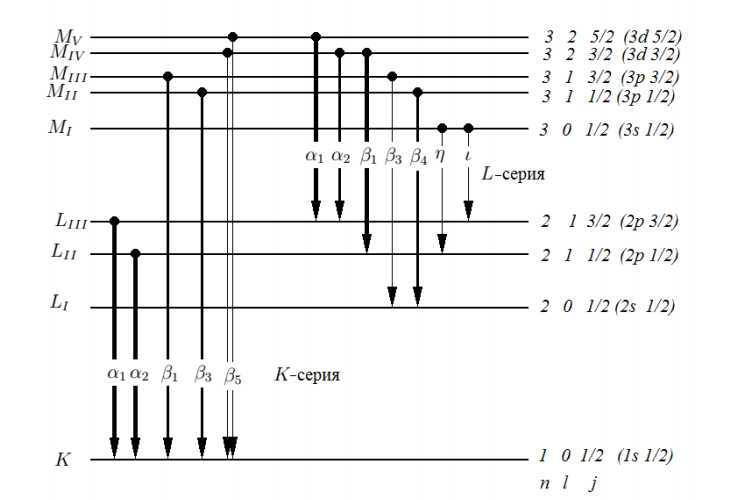
\includegraphics[width=15cm]{fig1.PNG}
\caption{Схема основных переходов $К$-серии и $L$-серии}
\label{ris:experimoriginal} %% метка рисунка для ссылки на него
\end{center}
\end{figure}

\section{Экспериментальная установка}

Для регистрации рентгеновских спектров характеристического излучения
в работе используется серийно выпускаемый рентгенофлуоресцентный
спектрометр «Спектроскан Макс-G». В состав прибора входят следующие
основные элементы: рентгеновская трубка, держатель образцов,
вогнутая пластина кристалла LiF, гониометр, а также пропорциональный
детектор. Схема прибора показана на рис. 2.

\begin{figure}[h]
\begin{center}
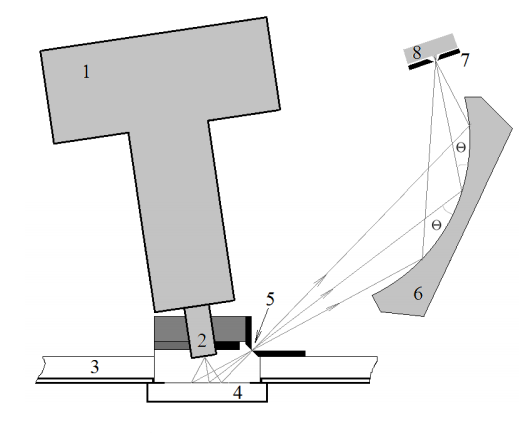
\includegraphics[width=8cm]{setup.PNG}
\caption{Схема рентгеновского спектрометра}
\label{ris:experimoriginal} %% метка рисунка для ссылки на него
\end{center}
\end{figure}

\section{Выполнение работы}
\begin{enumerate}
    \item Cнимем спектры характеристического излучения для различных элементов. Результаты измерений занесём в таблицу 1. Графики спектров представим на рис. 3 - 12 (пик слева отвечает переходу $K_{\beta}$)


    \begin{figure}[h]
\begin{center}
\begin{minipage}[h]{0.45\linewidth}
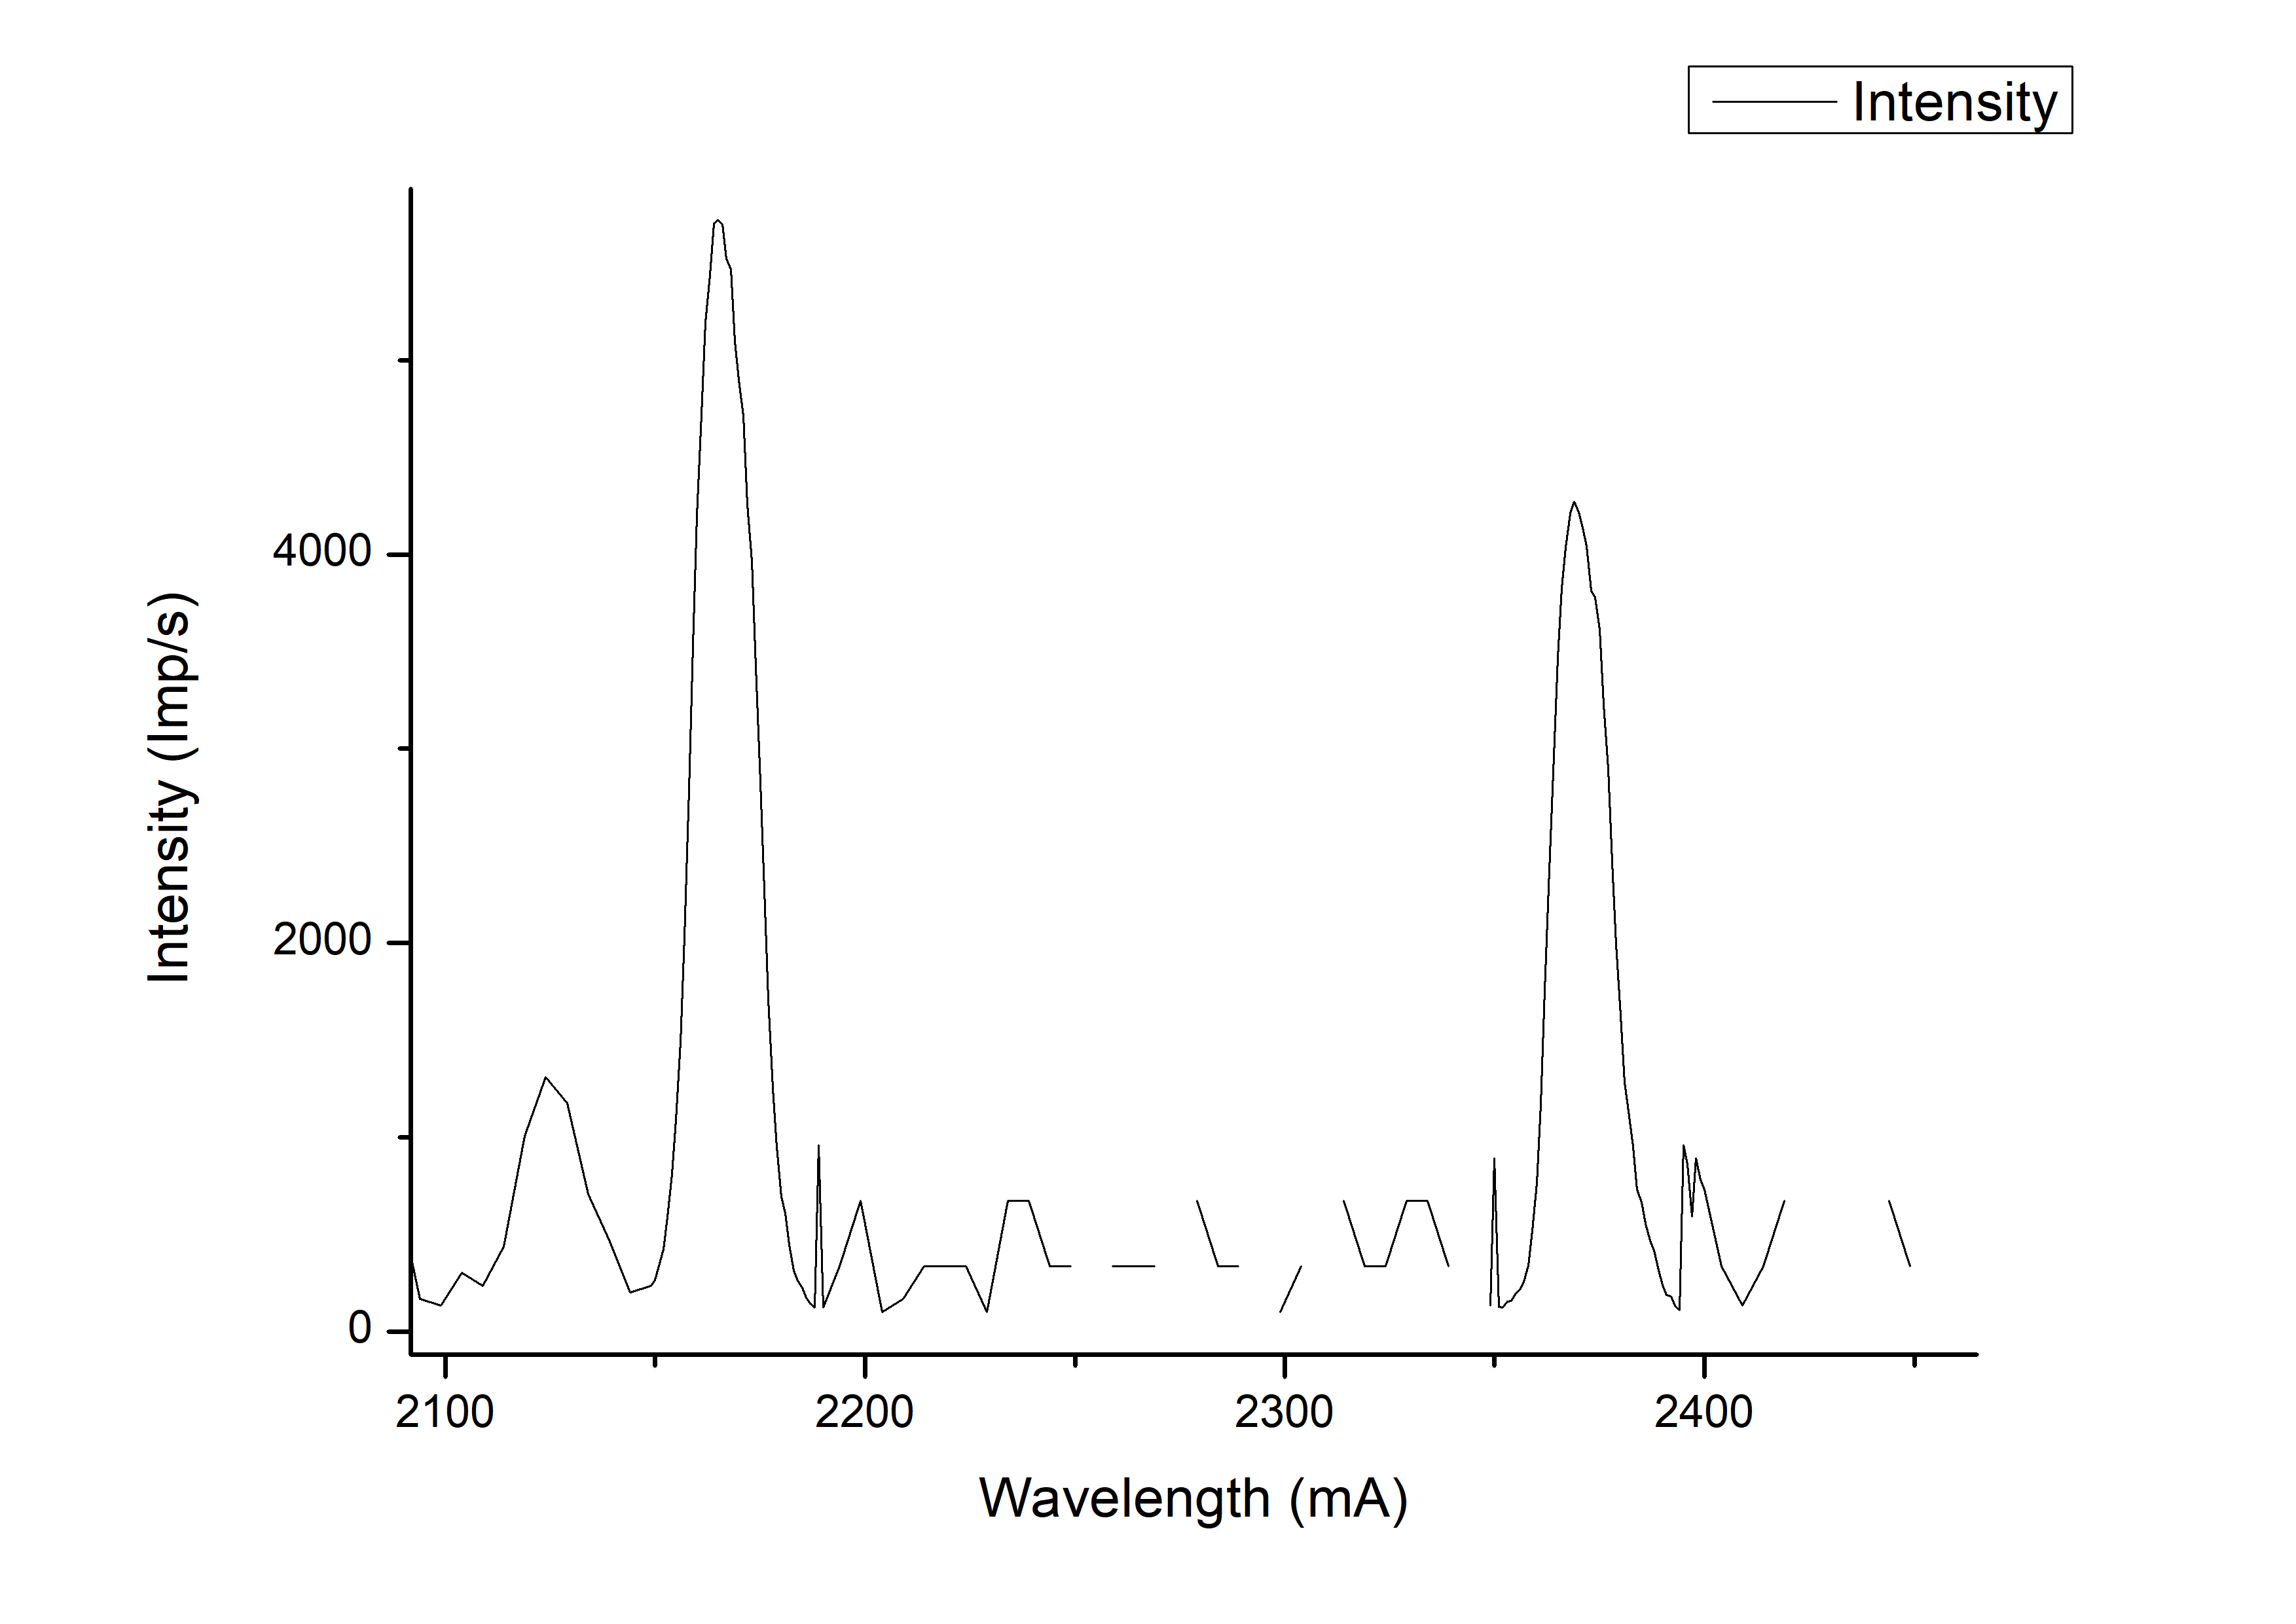
\includegraphics[width=1\linewidth]{Nd.png}
\caption{Спектр характеристического излучения неодима $^{60}$Nd} %% подпись к рисунку\label{ris:experimoriginal} %% метка рисунка для ссылки на него
\end{minipage}
\hfill 
\begin{minipage}[h]{0.45\linewidth}
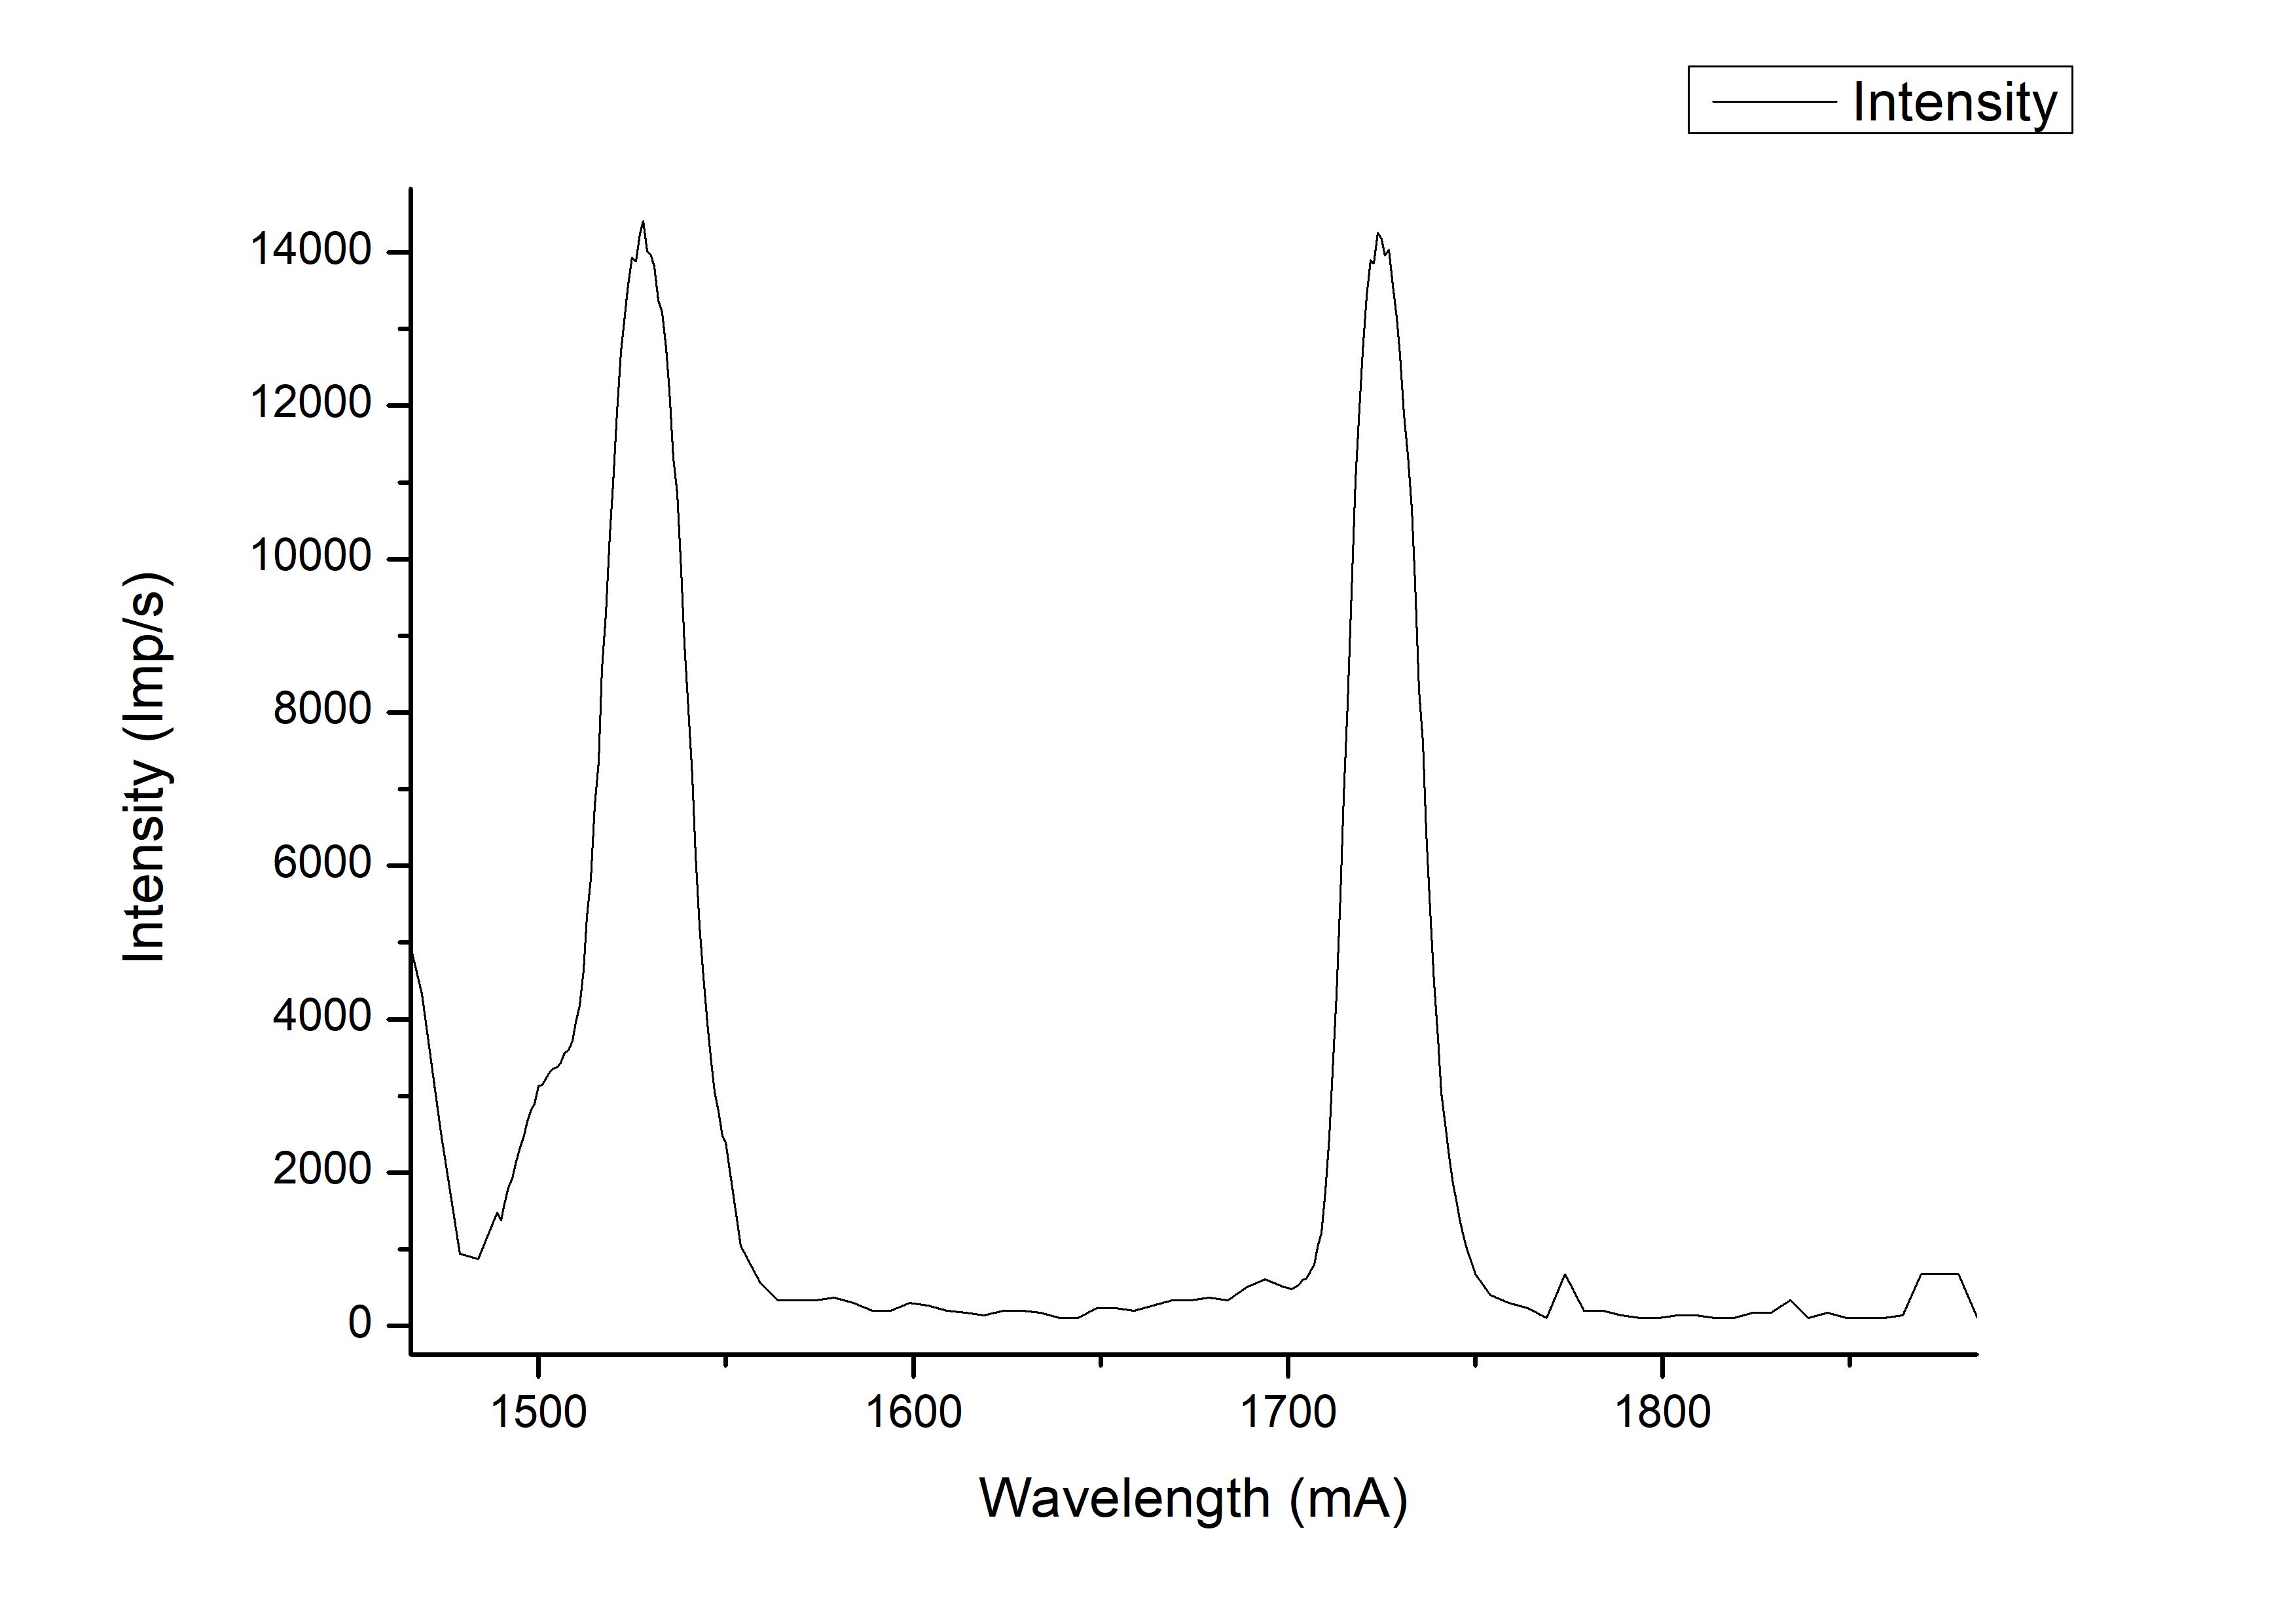
\includegraphics[width=1\linewidth]{Tm.png}
\caption{Спектр характеристического излучения тулия $^{69}$Tm}
\label{ris:experimcoded}
\end{minipage}
\end{center}
\end{figure}


    \begin{figure}[h]
\begin{center}
\begin{minipage}[h]{0.45\linewidth}
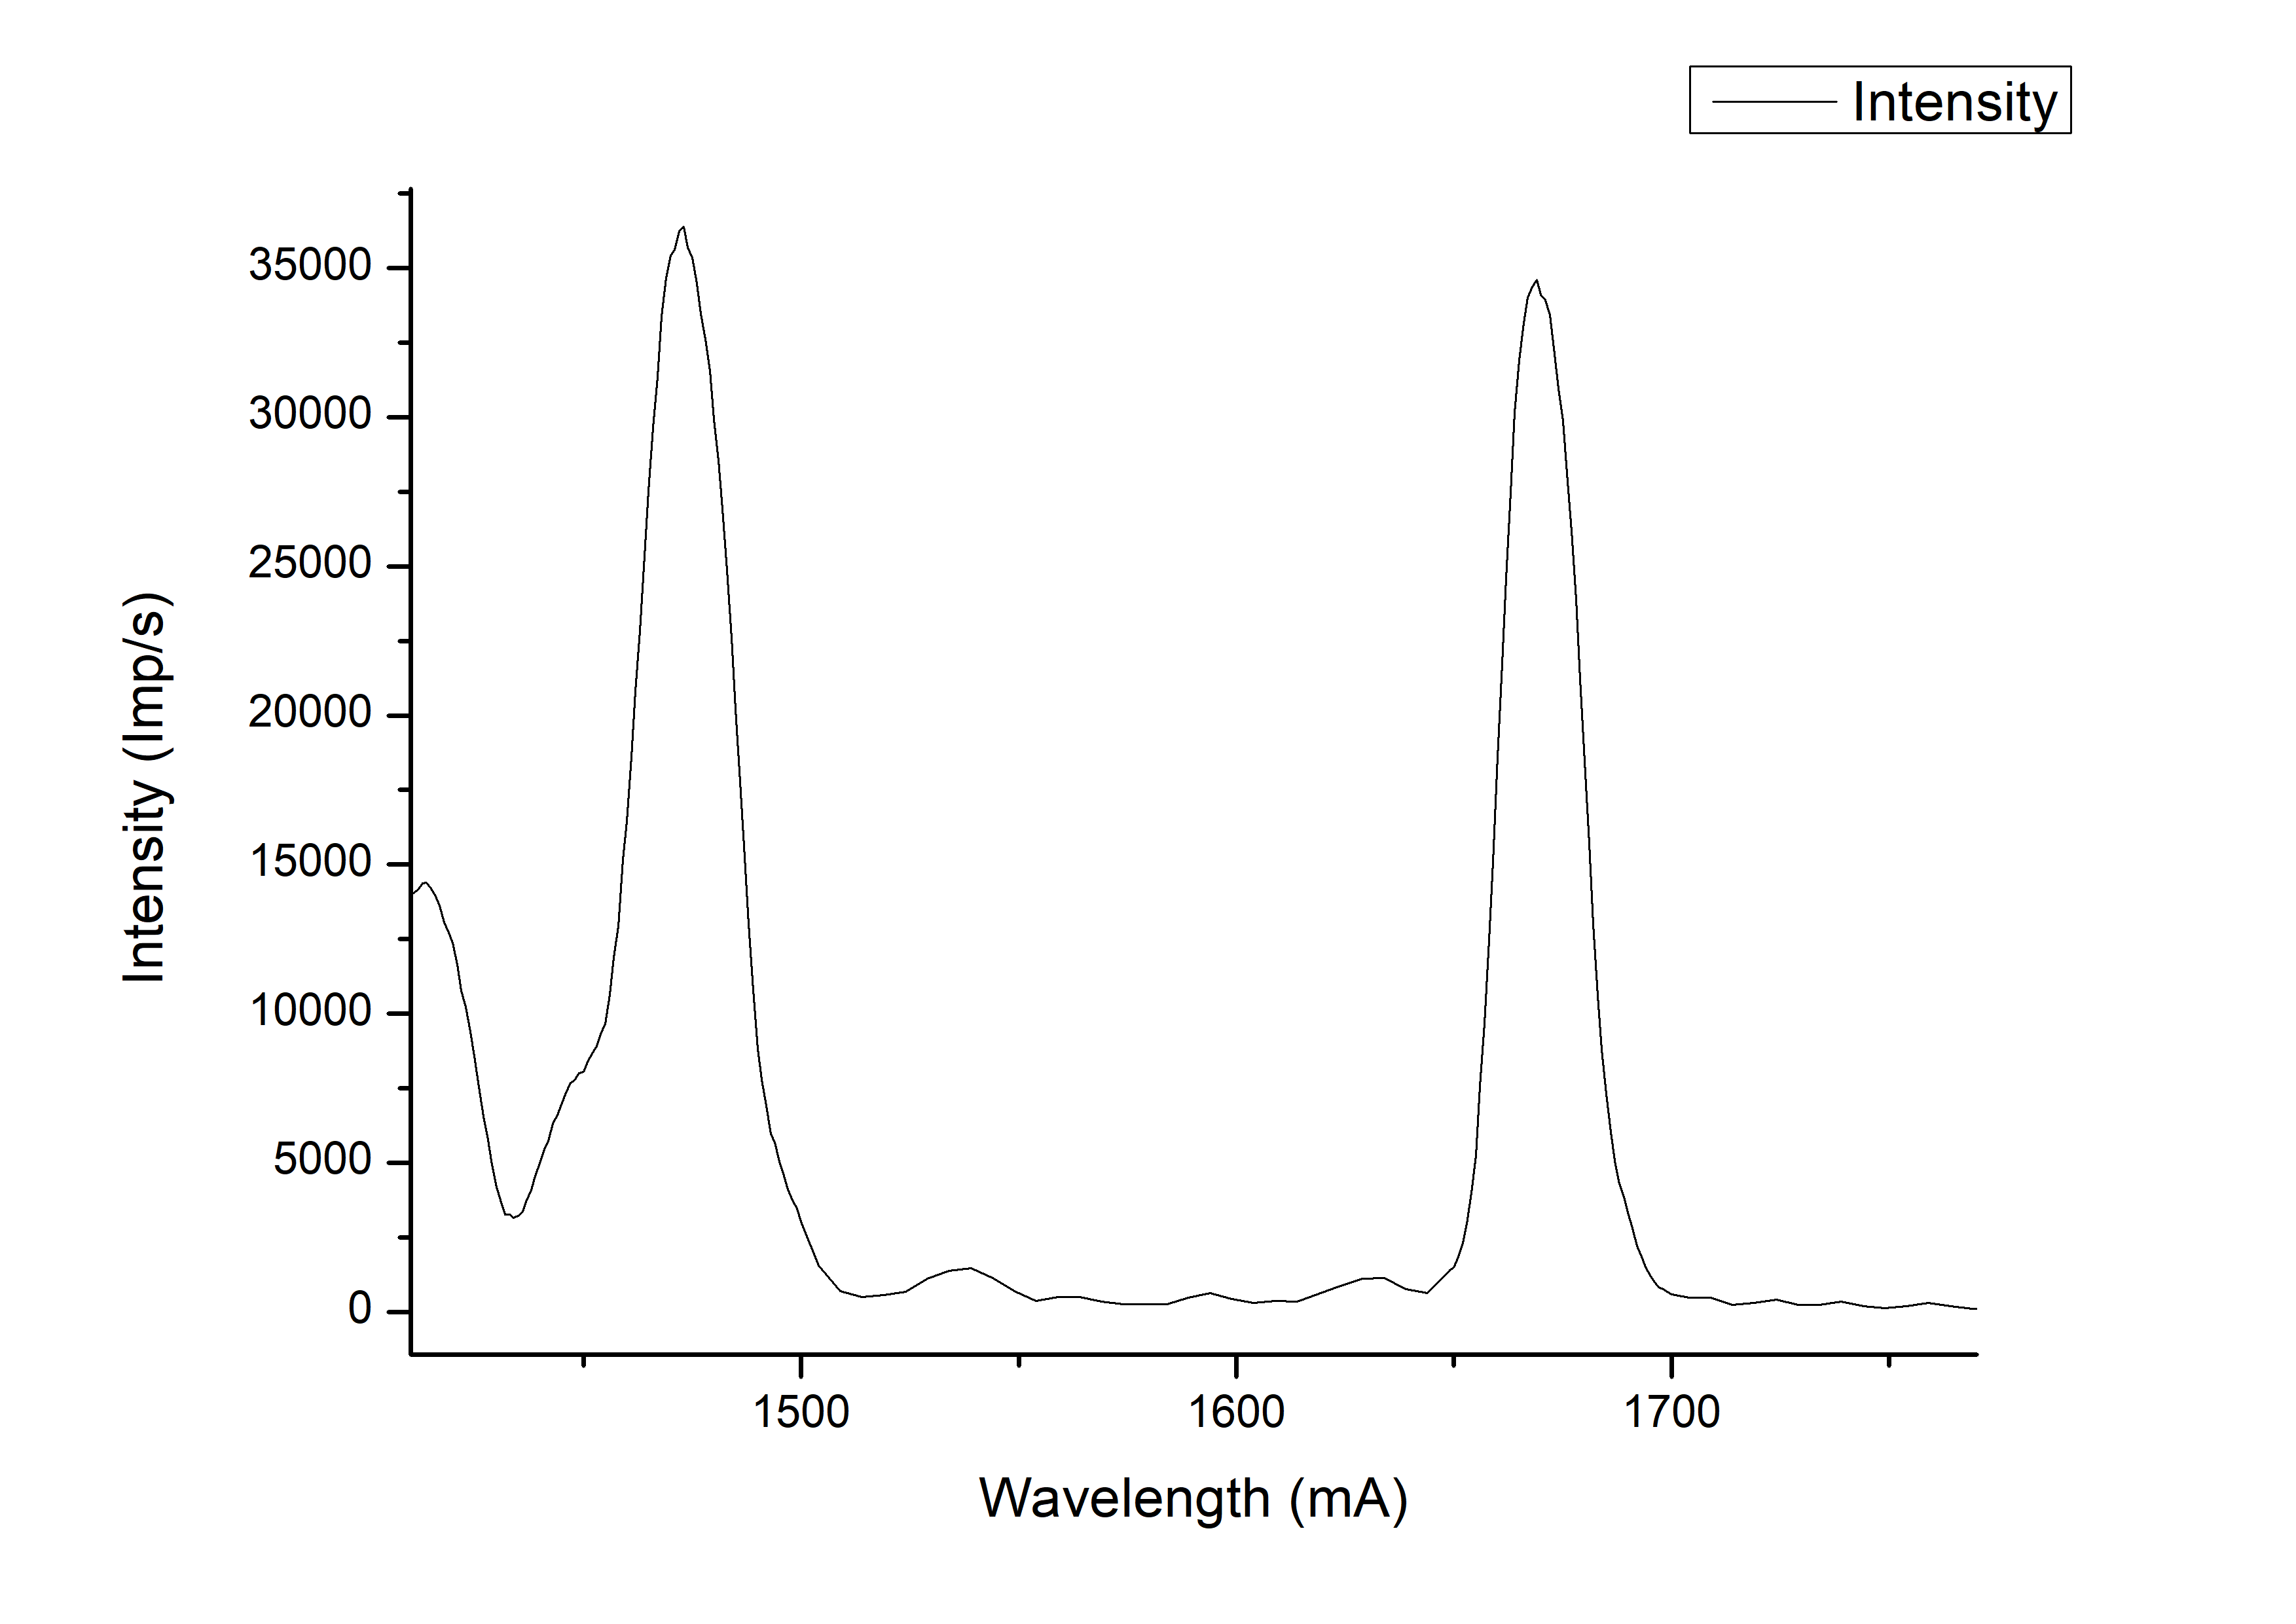
\includegraphics[width=1\linewidth]{Yb.png}
\caption{Спектр характеристического излучения иттербия $^{70}$Yb} %% подпись к рисунку\label{ris:experimoriginal} %% метка рисунка для ссылки на него
\end{minipage}
\hfill 
\begin{minipage}[h]{0.45\linewidth}
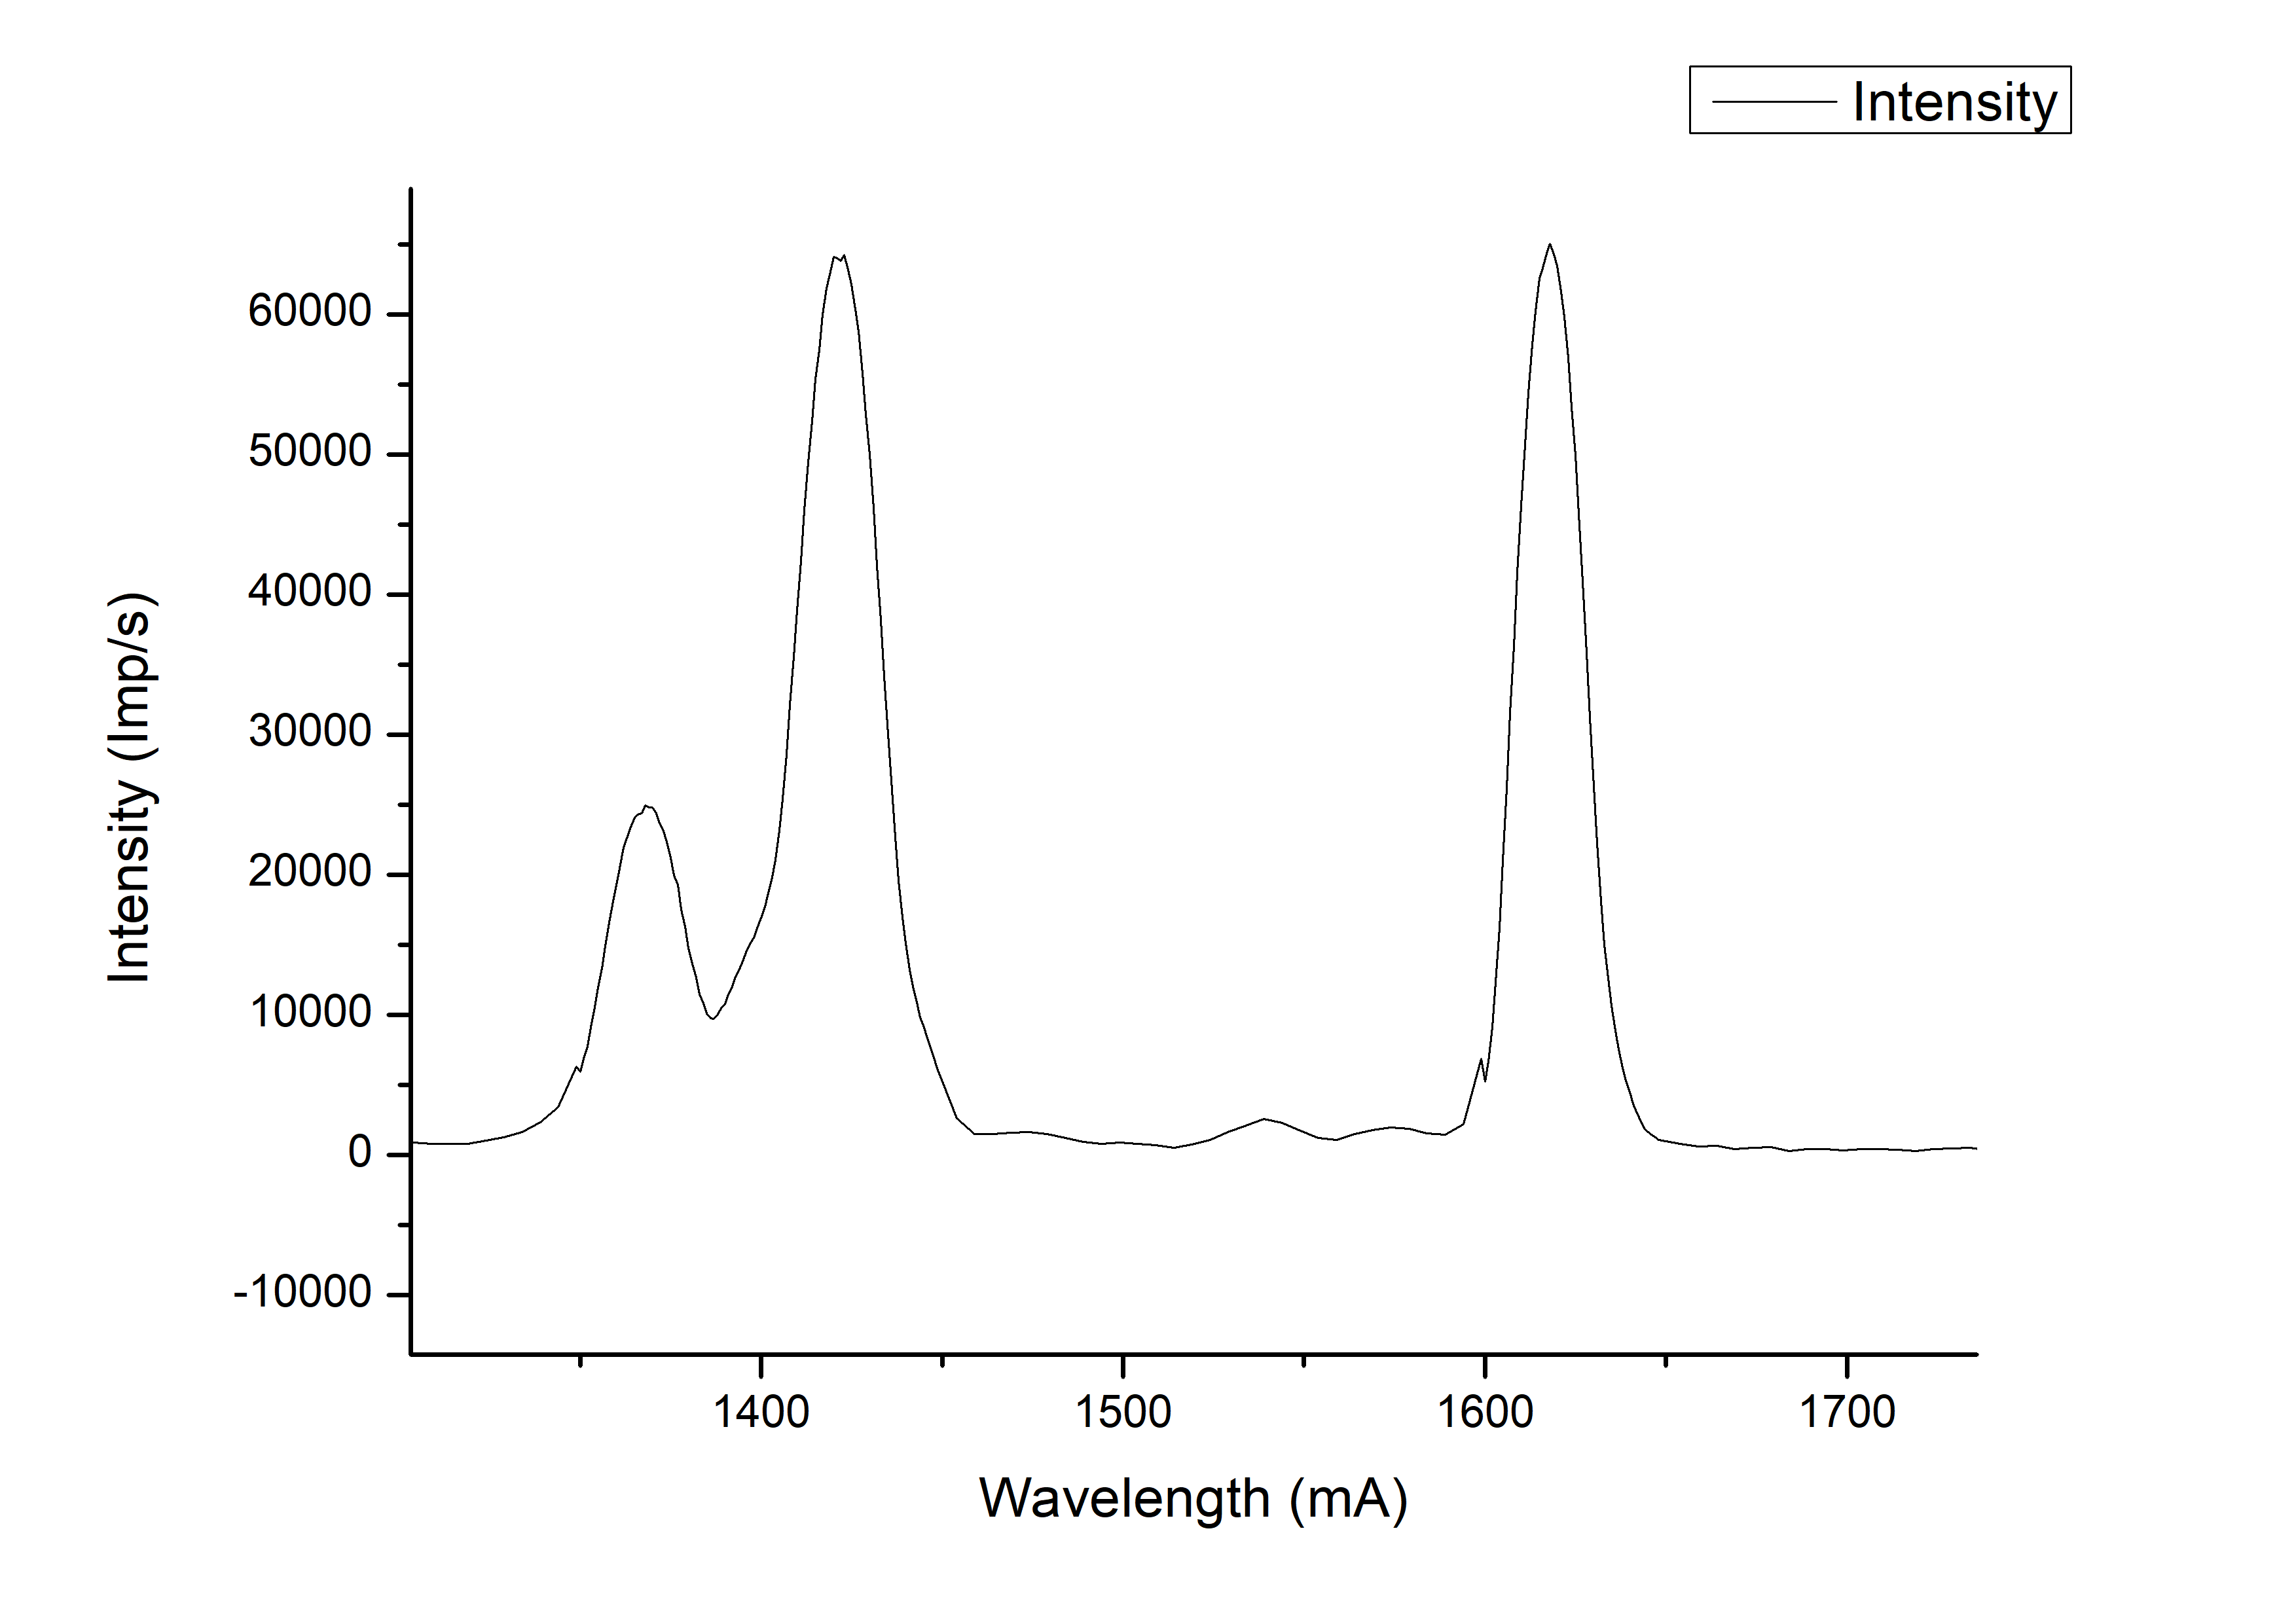
\includegraphics[width=1\linewidth]{Lu.png}
\caption{Спектр характеристического излучения лютеция $^{71}$Lu}
\label{ris:experimcoded}
\end{minipage}
\end{center}
\end{figure}

    \begin{figure}[h]
\begin{center}
\begin{minipage}[h]{0.45\linewidth}
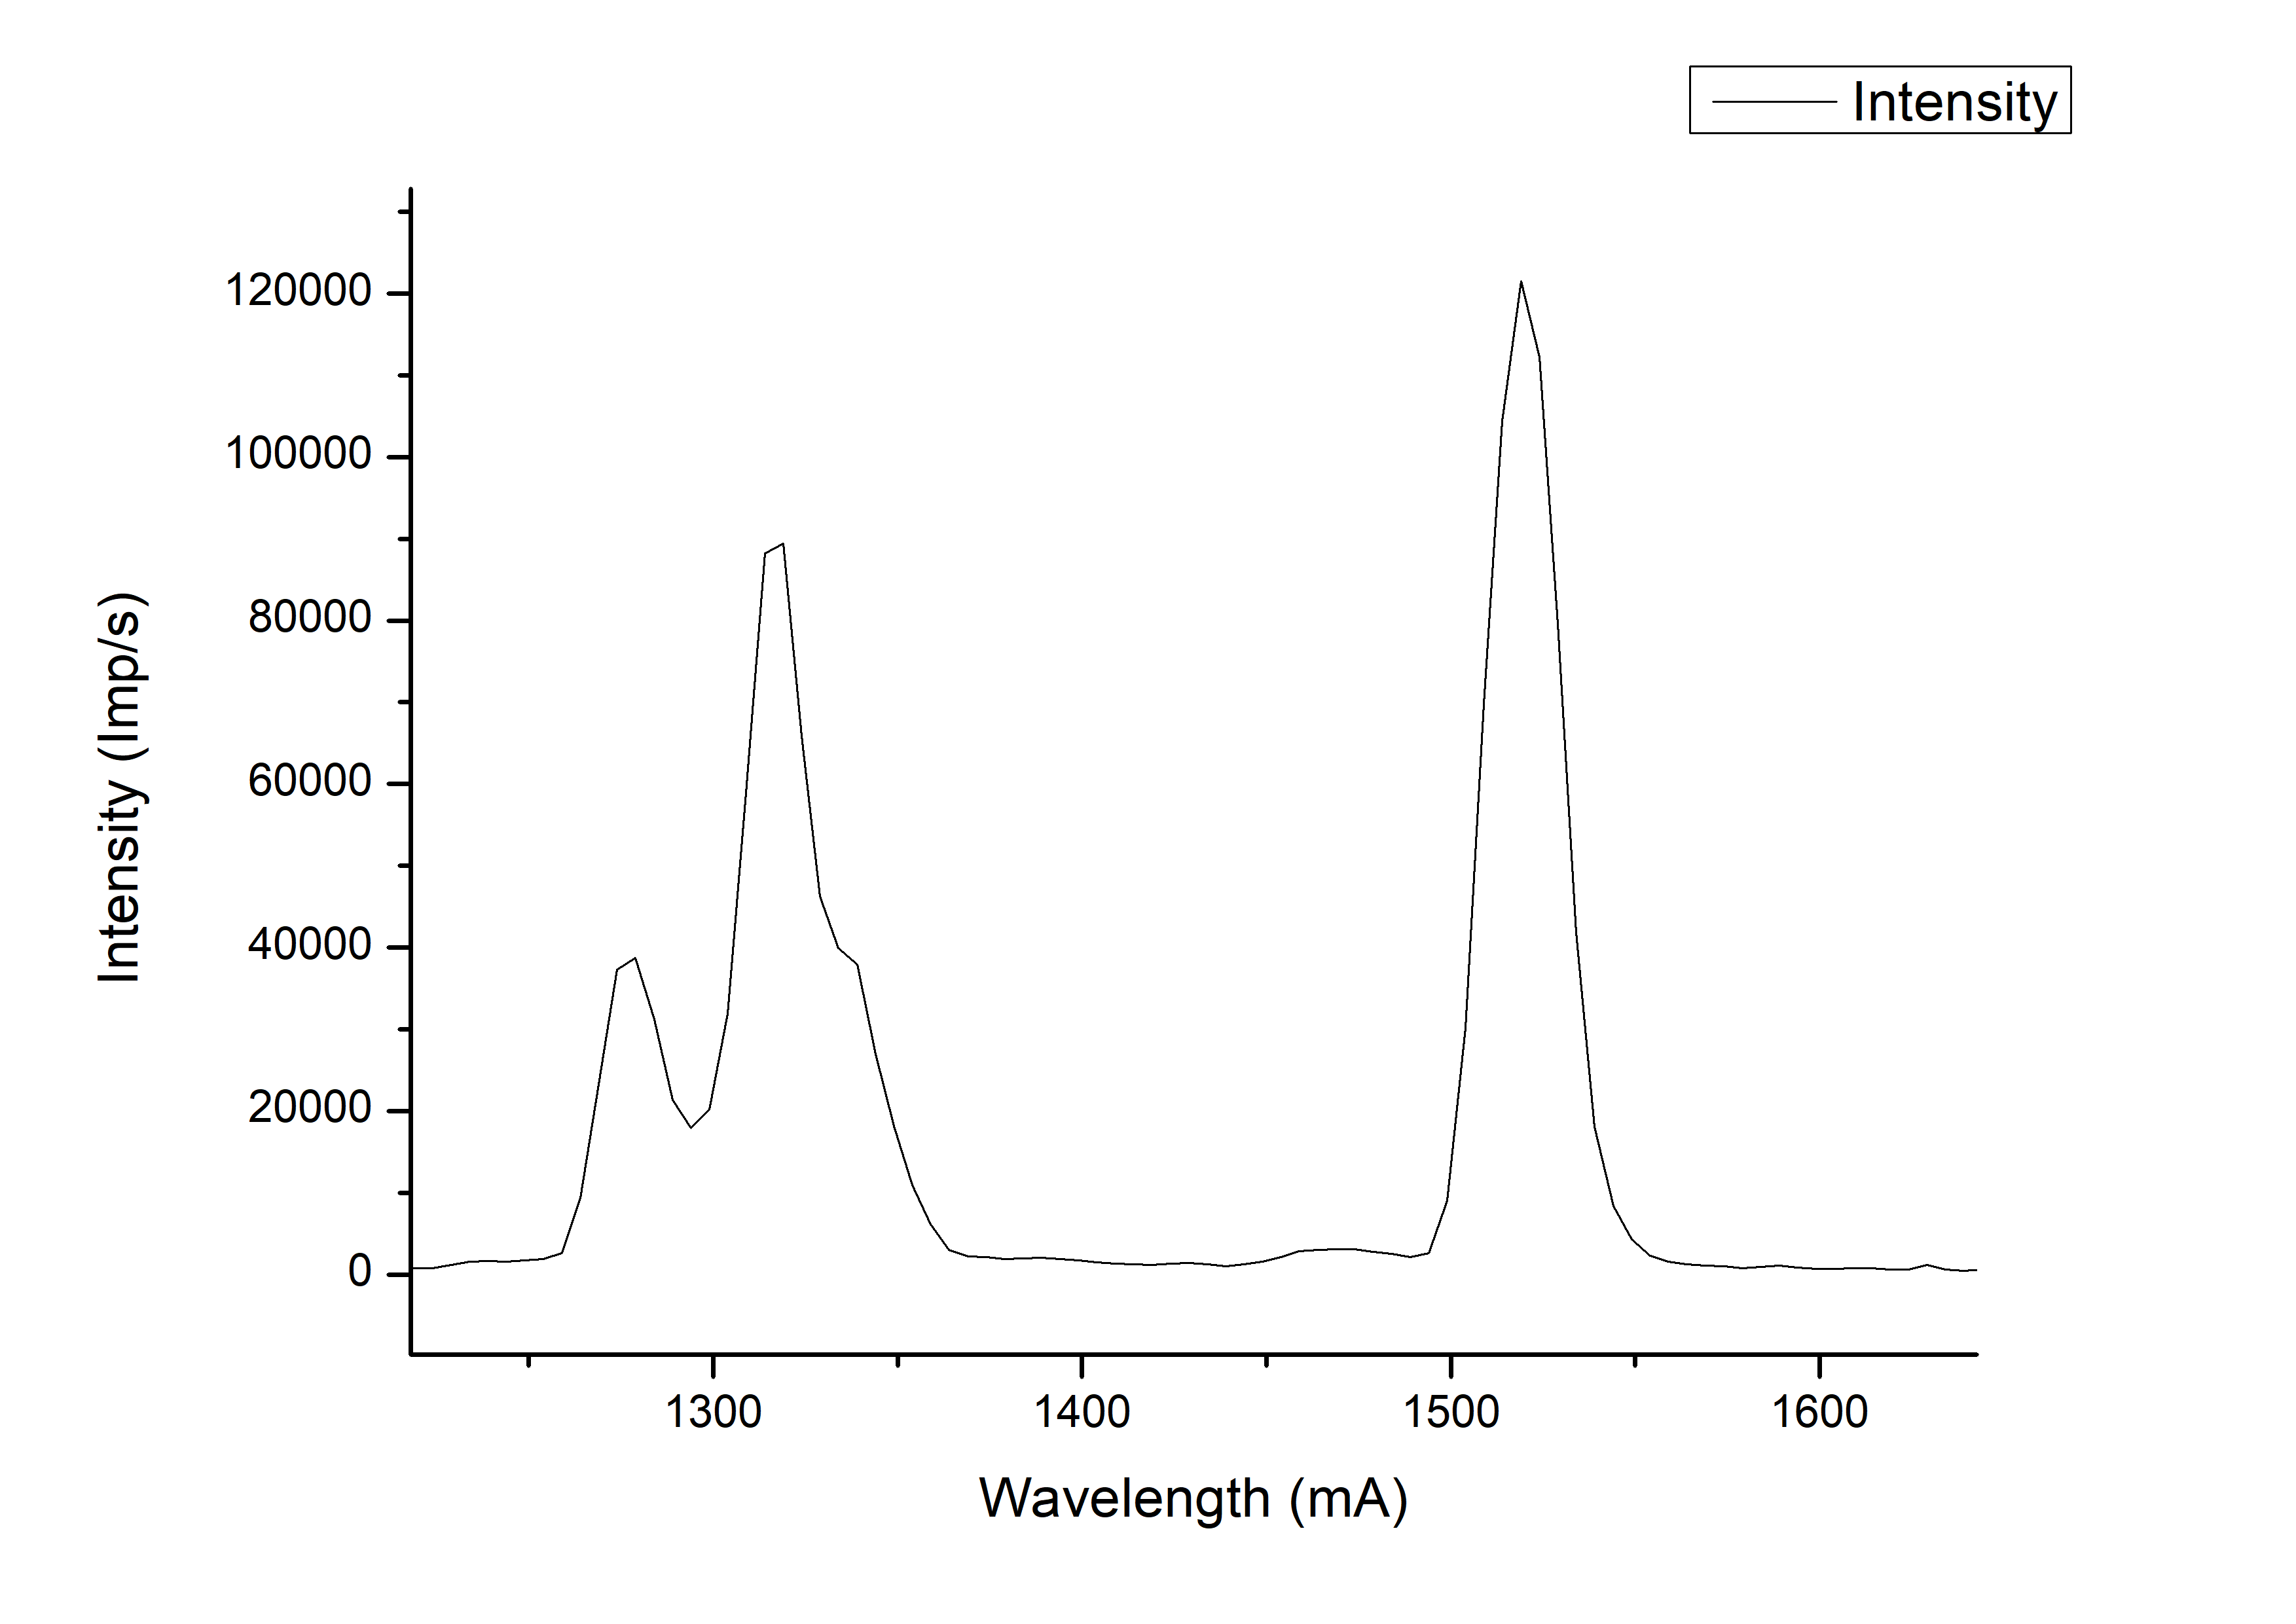
\includegraphics[width=1\linewidth]{Ta.png}
\caption{Спектр характеристического излучения тантала $^{73}$Ta} %% подпись к рисунку\label{ris:experimoriginal} %% метка рисунка для ссылки на него
\end{minipage}
\hfill 
\begin{minipage}[h]{0.45\linewidth}
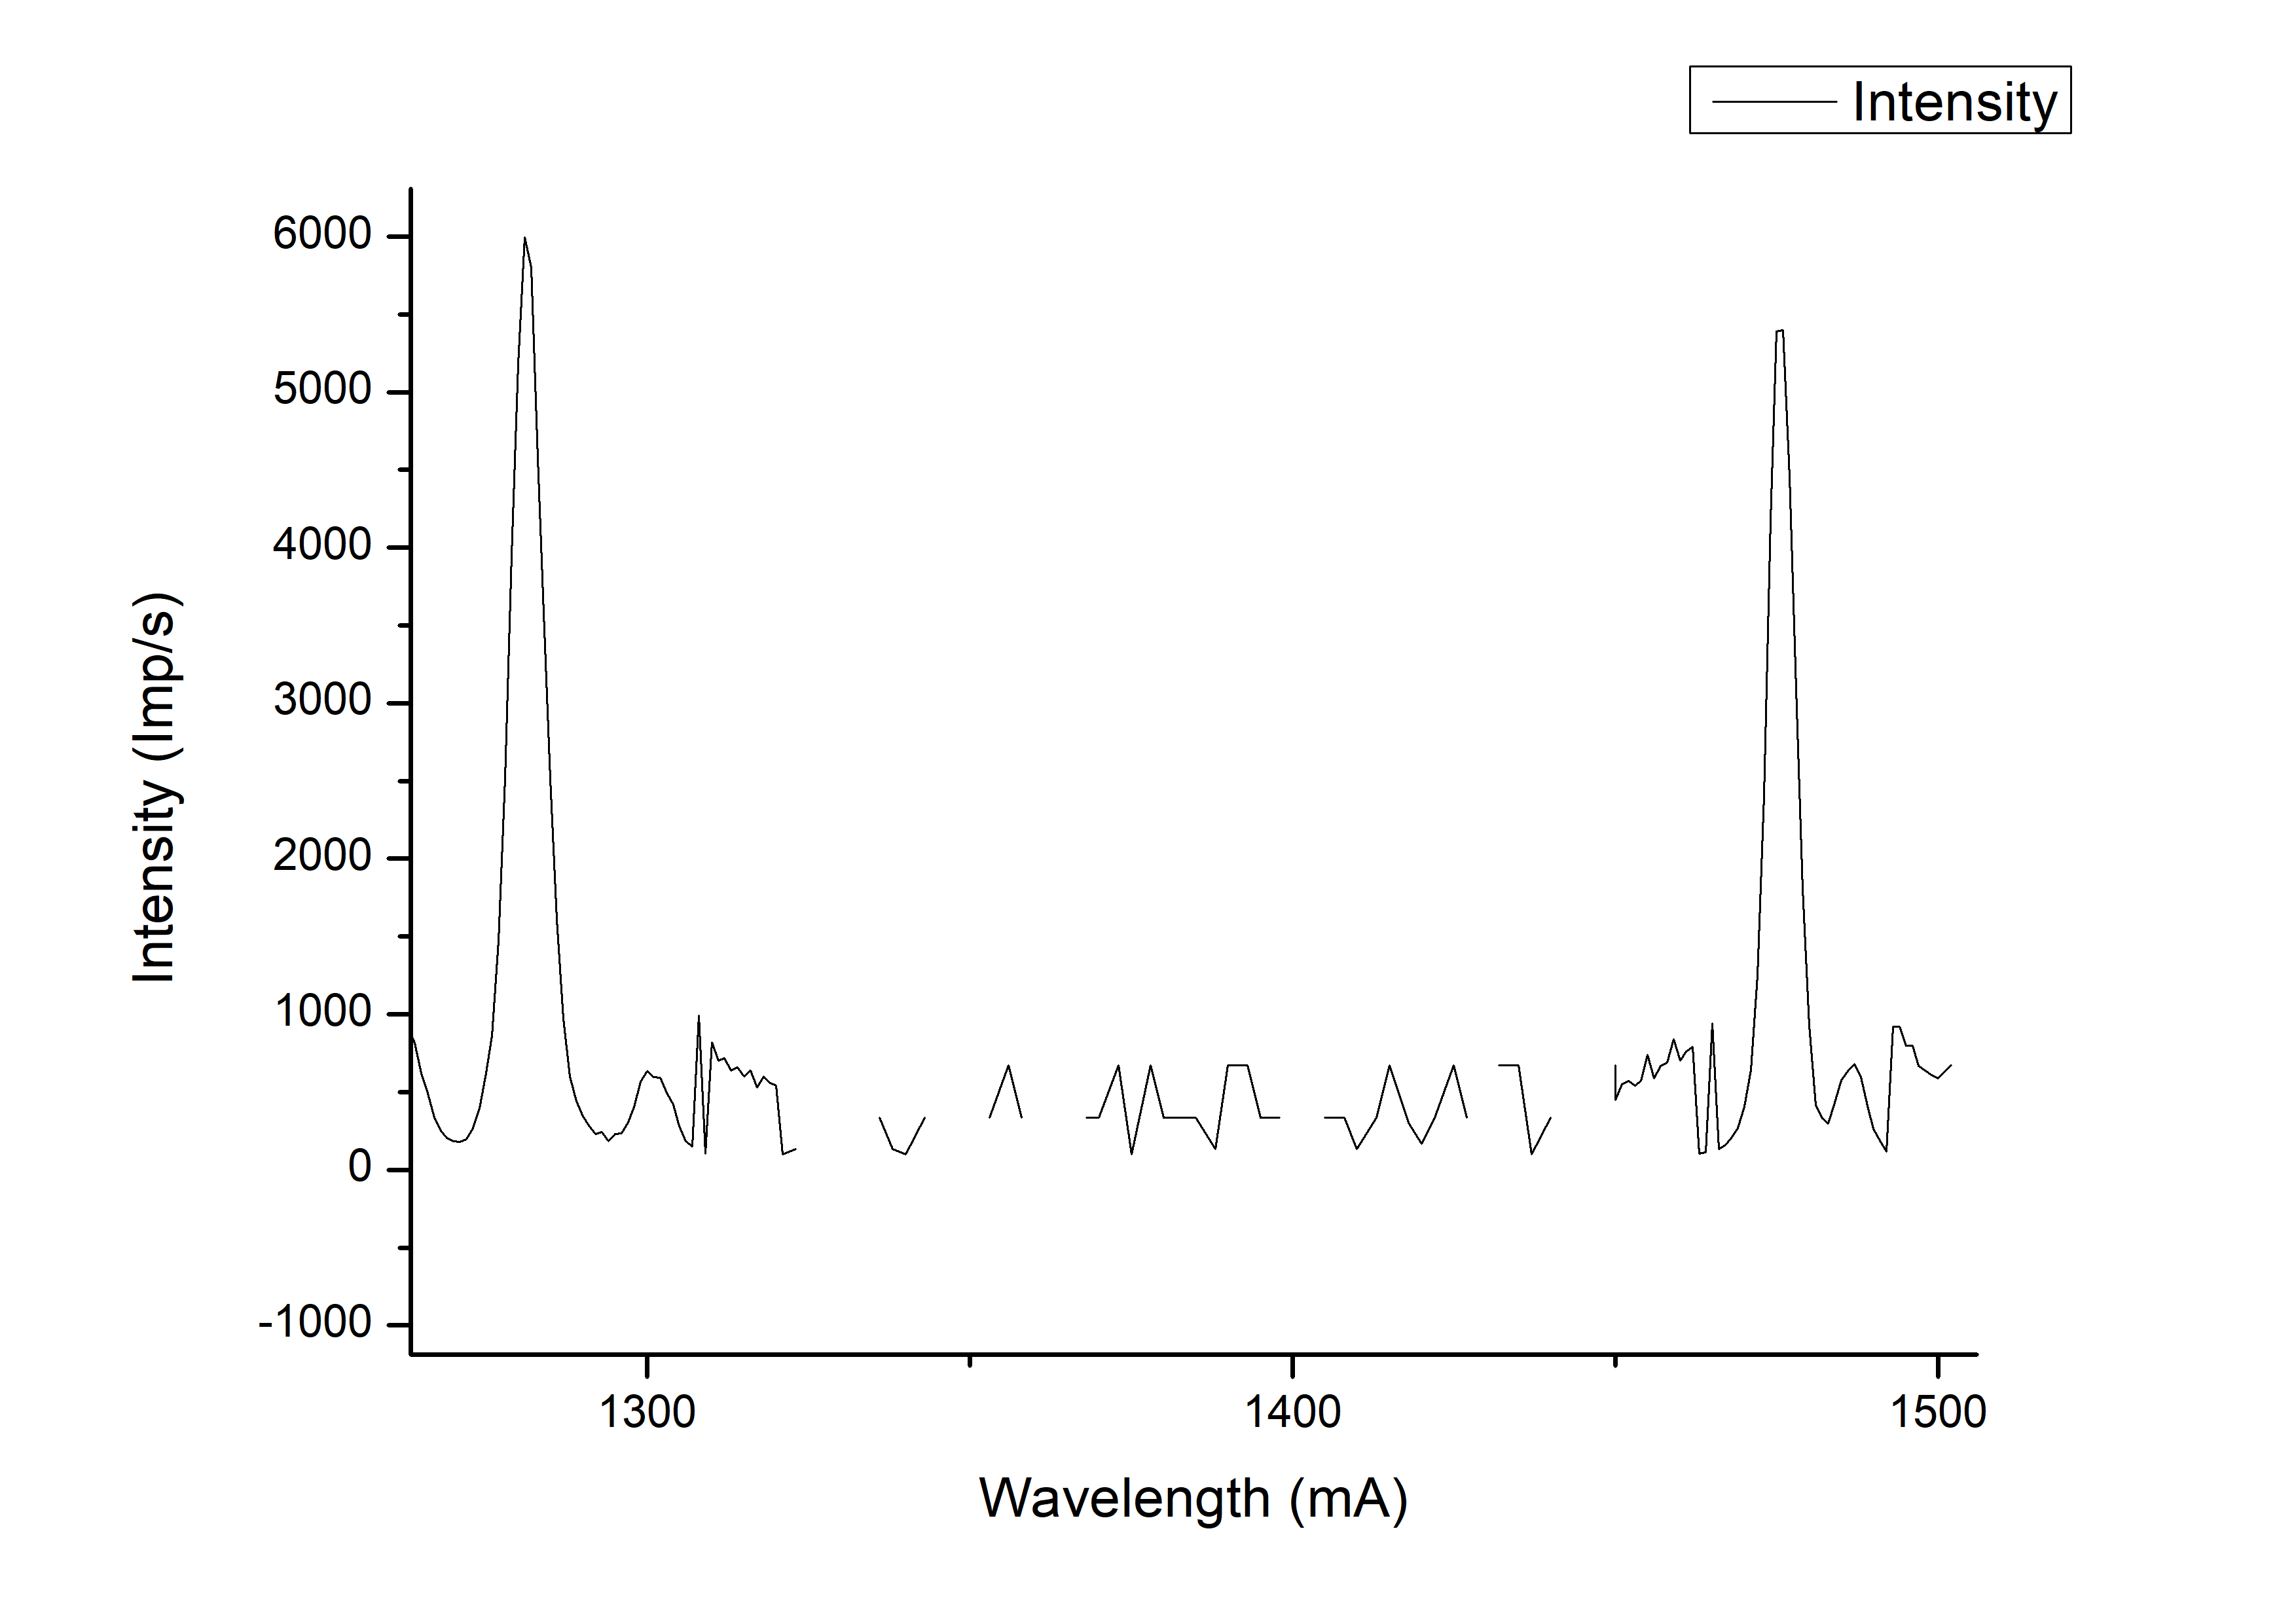
\includegraphics[width=1\linewidth]{W.png}
\caption{Спектр характеристического излучения вольфрама $^{74}$W}
\label{ris:experimcoded}
\end{minipage}
\end{center}
\end{figure}

    \begin{figure}[h]
\begin{center}
\begin{minipage}[h]{0.45\linewidth}
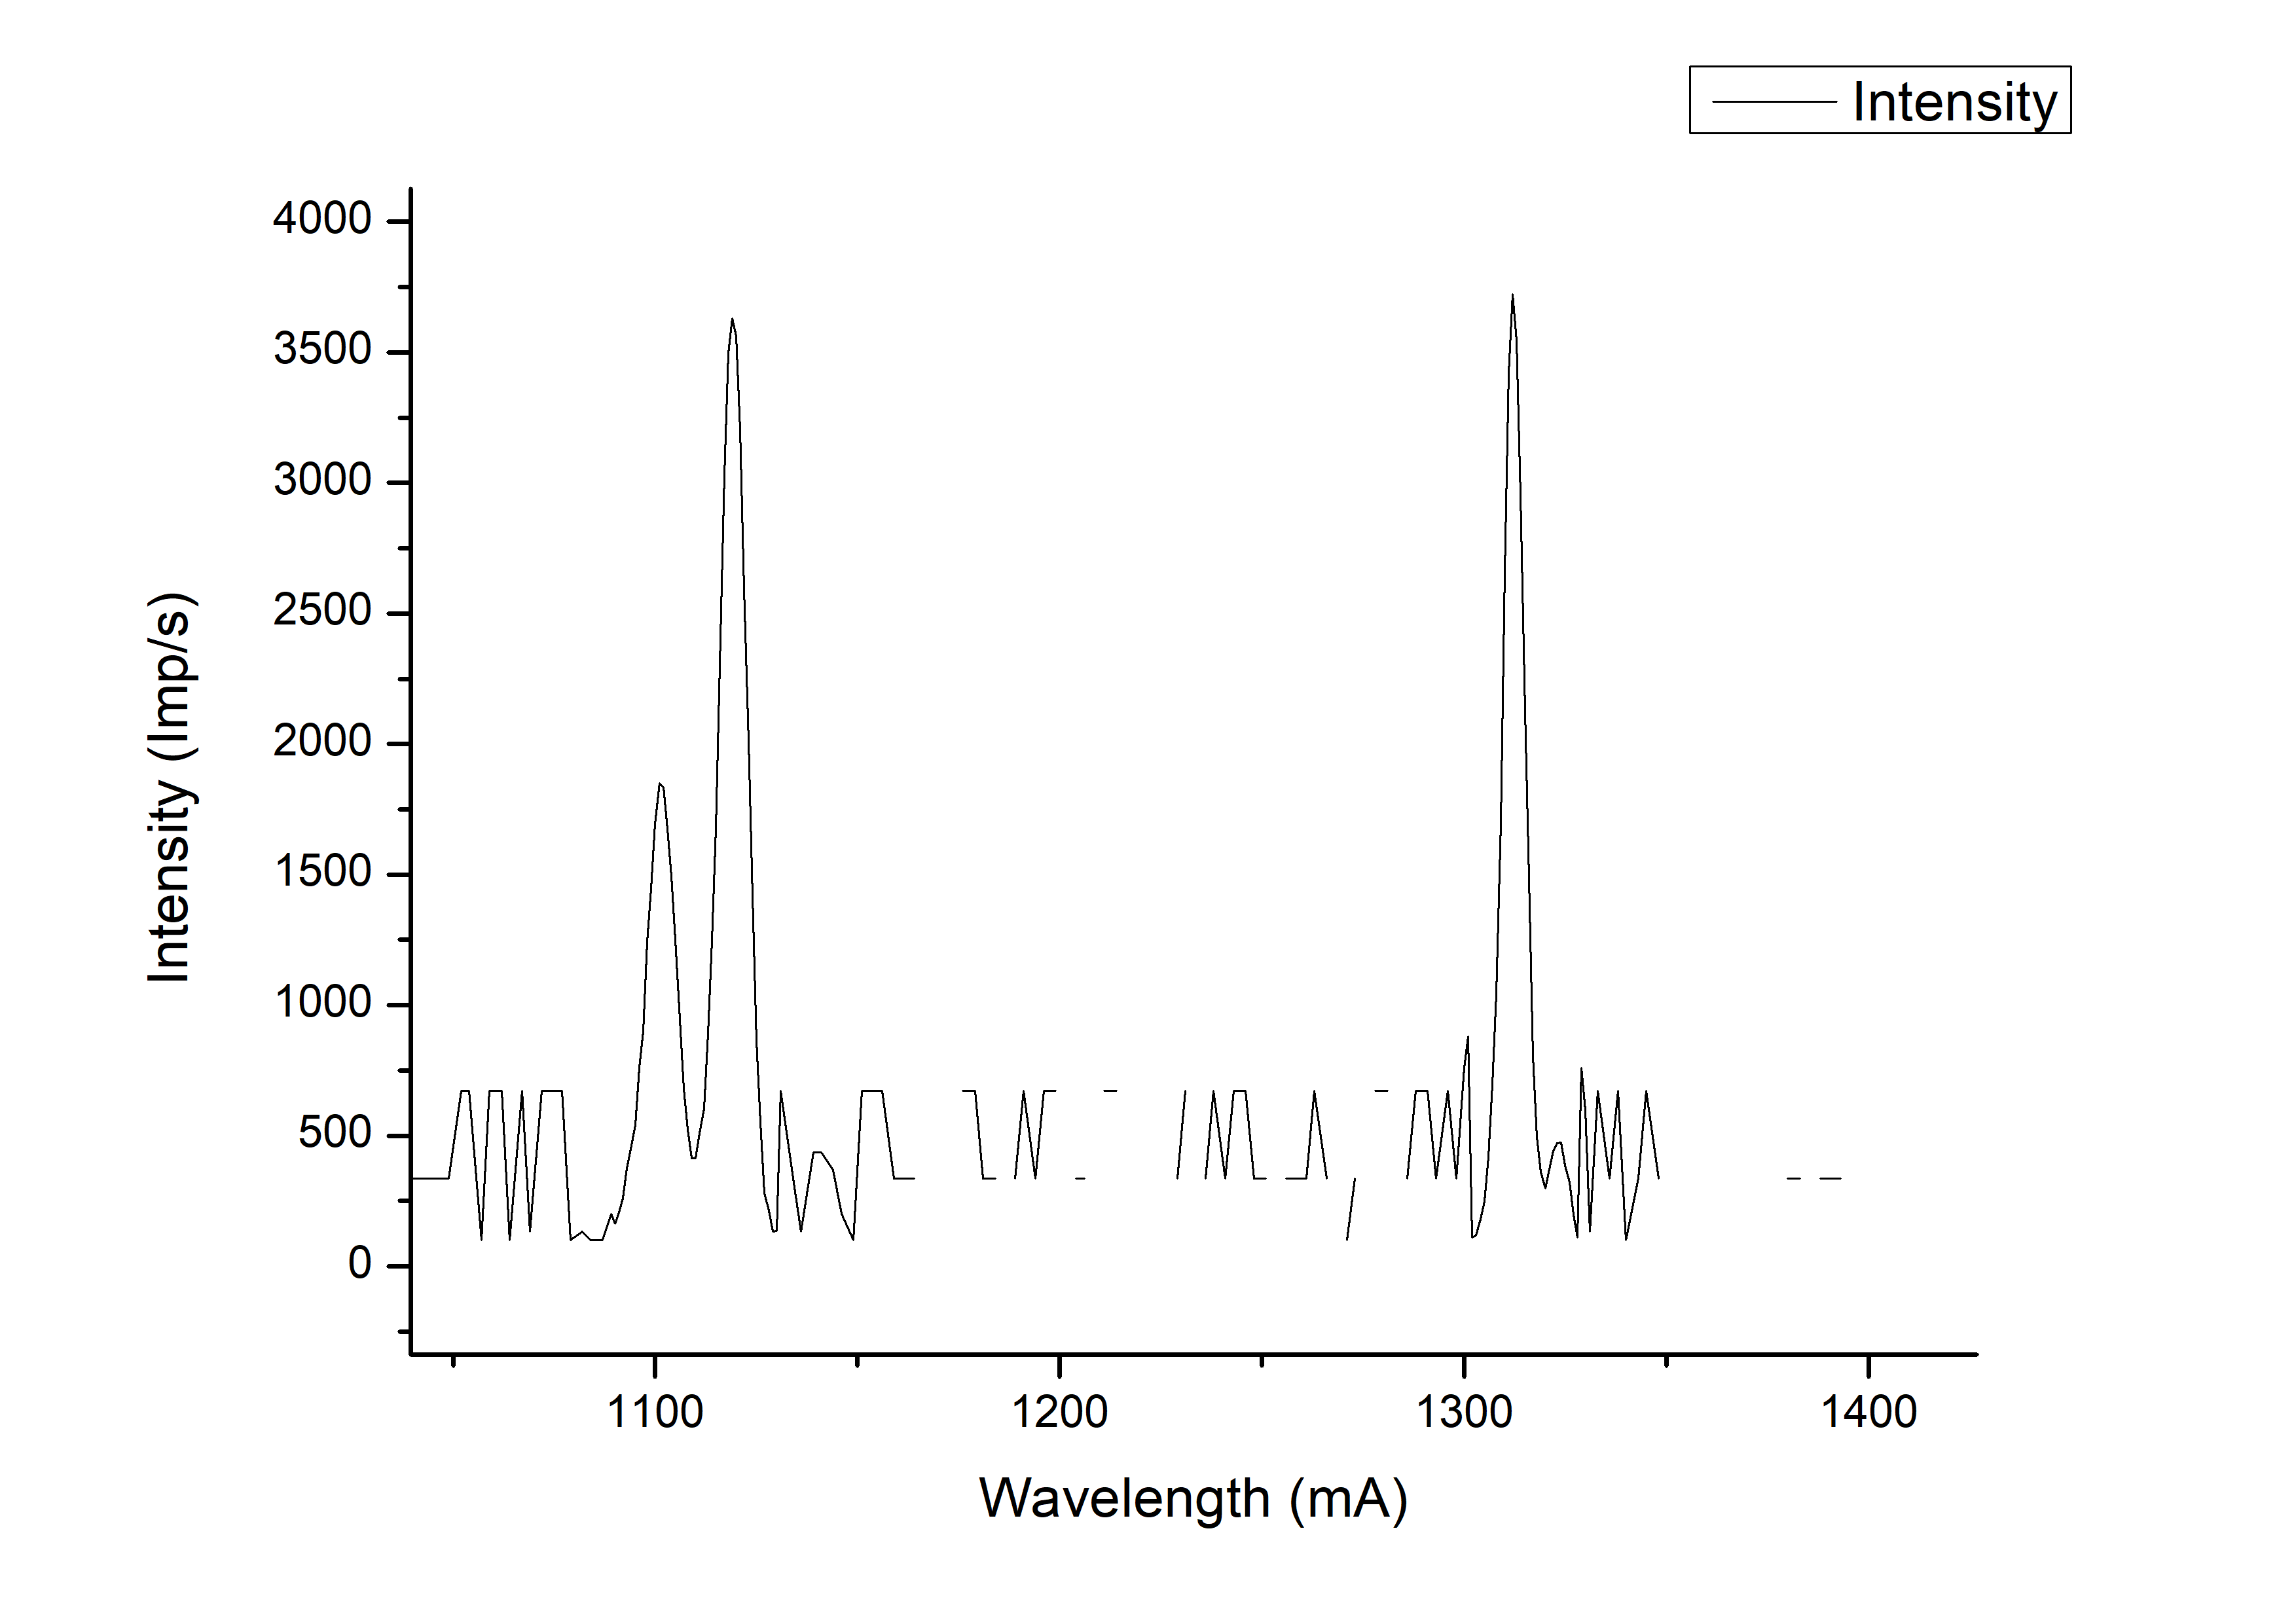
\includegraphics[width=1\linewidth]{Pt.png}
\caption{Спектр характеристического излучения платины $^{78}$Pt} %% подпись к рисунку\label{ris:experimoriginal} %% метка рисунка для ссылки на него
\end{minipage}
\hfill 
\begin{minipage}[h]{0.45\linewidth}
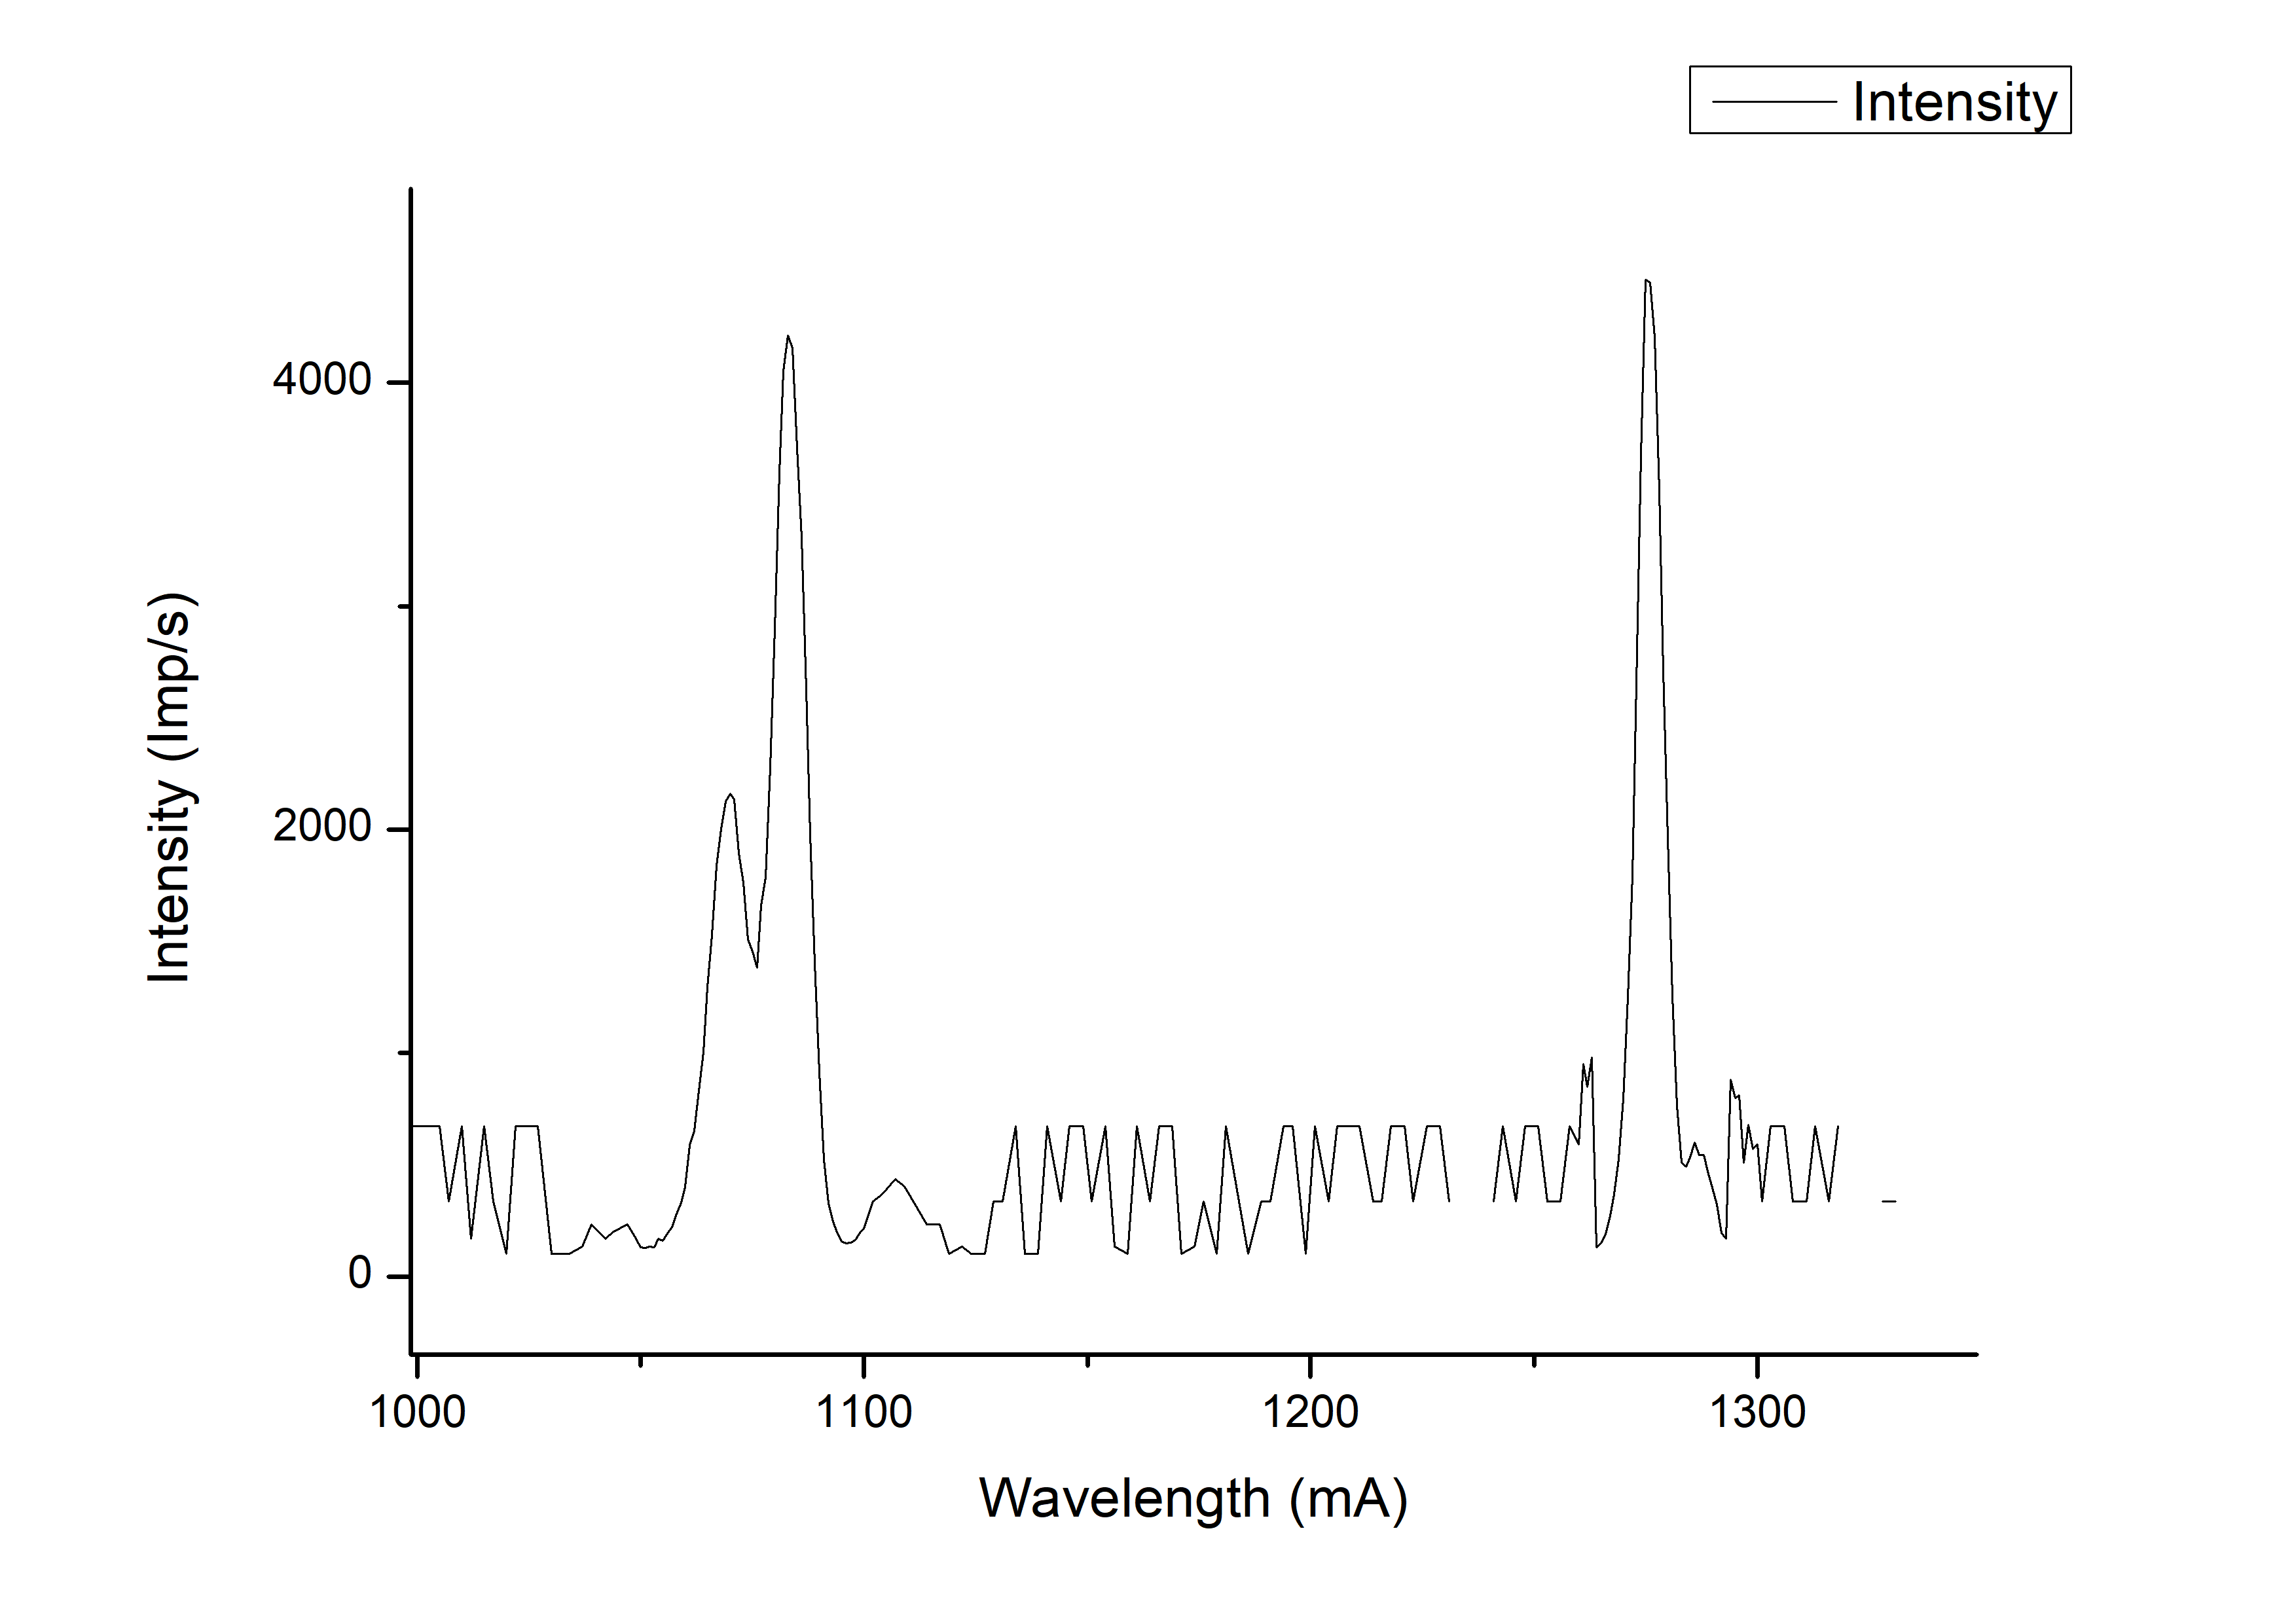
\includegraphics[width=1\linewidth]{Au.png}
\caption{Спектр характеристического излучения золота $^{79}$Au}
\label{ris:experimcoded}
\end{minipage}
\end{center}
\end{figure}


    \begin{figure}[h]
\begin{center}
\begin{minipage}[h]{0.45\linewidth}
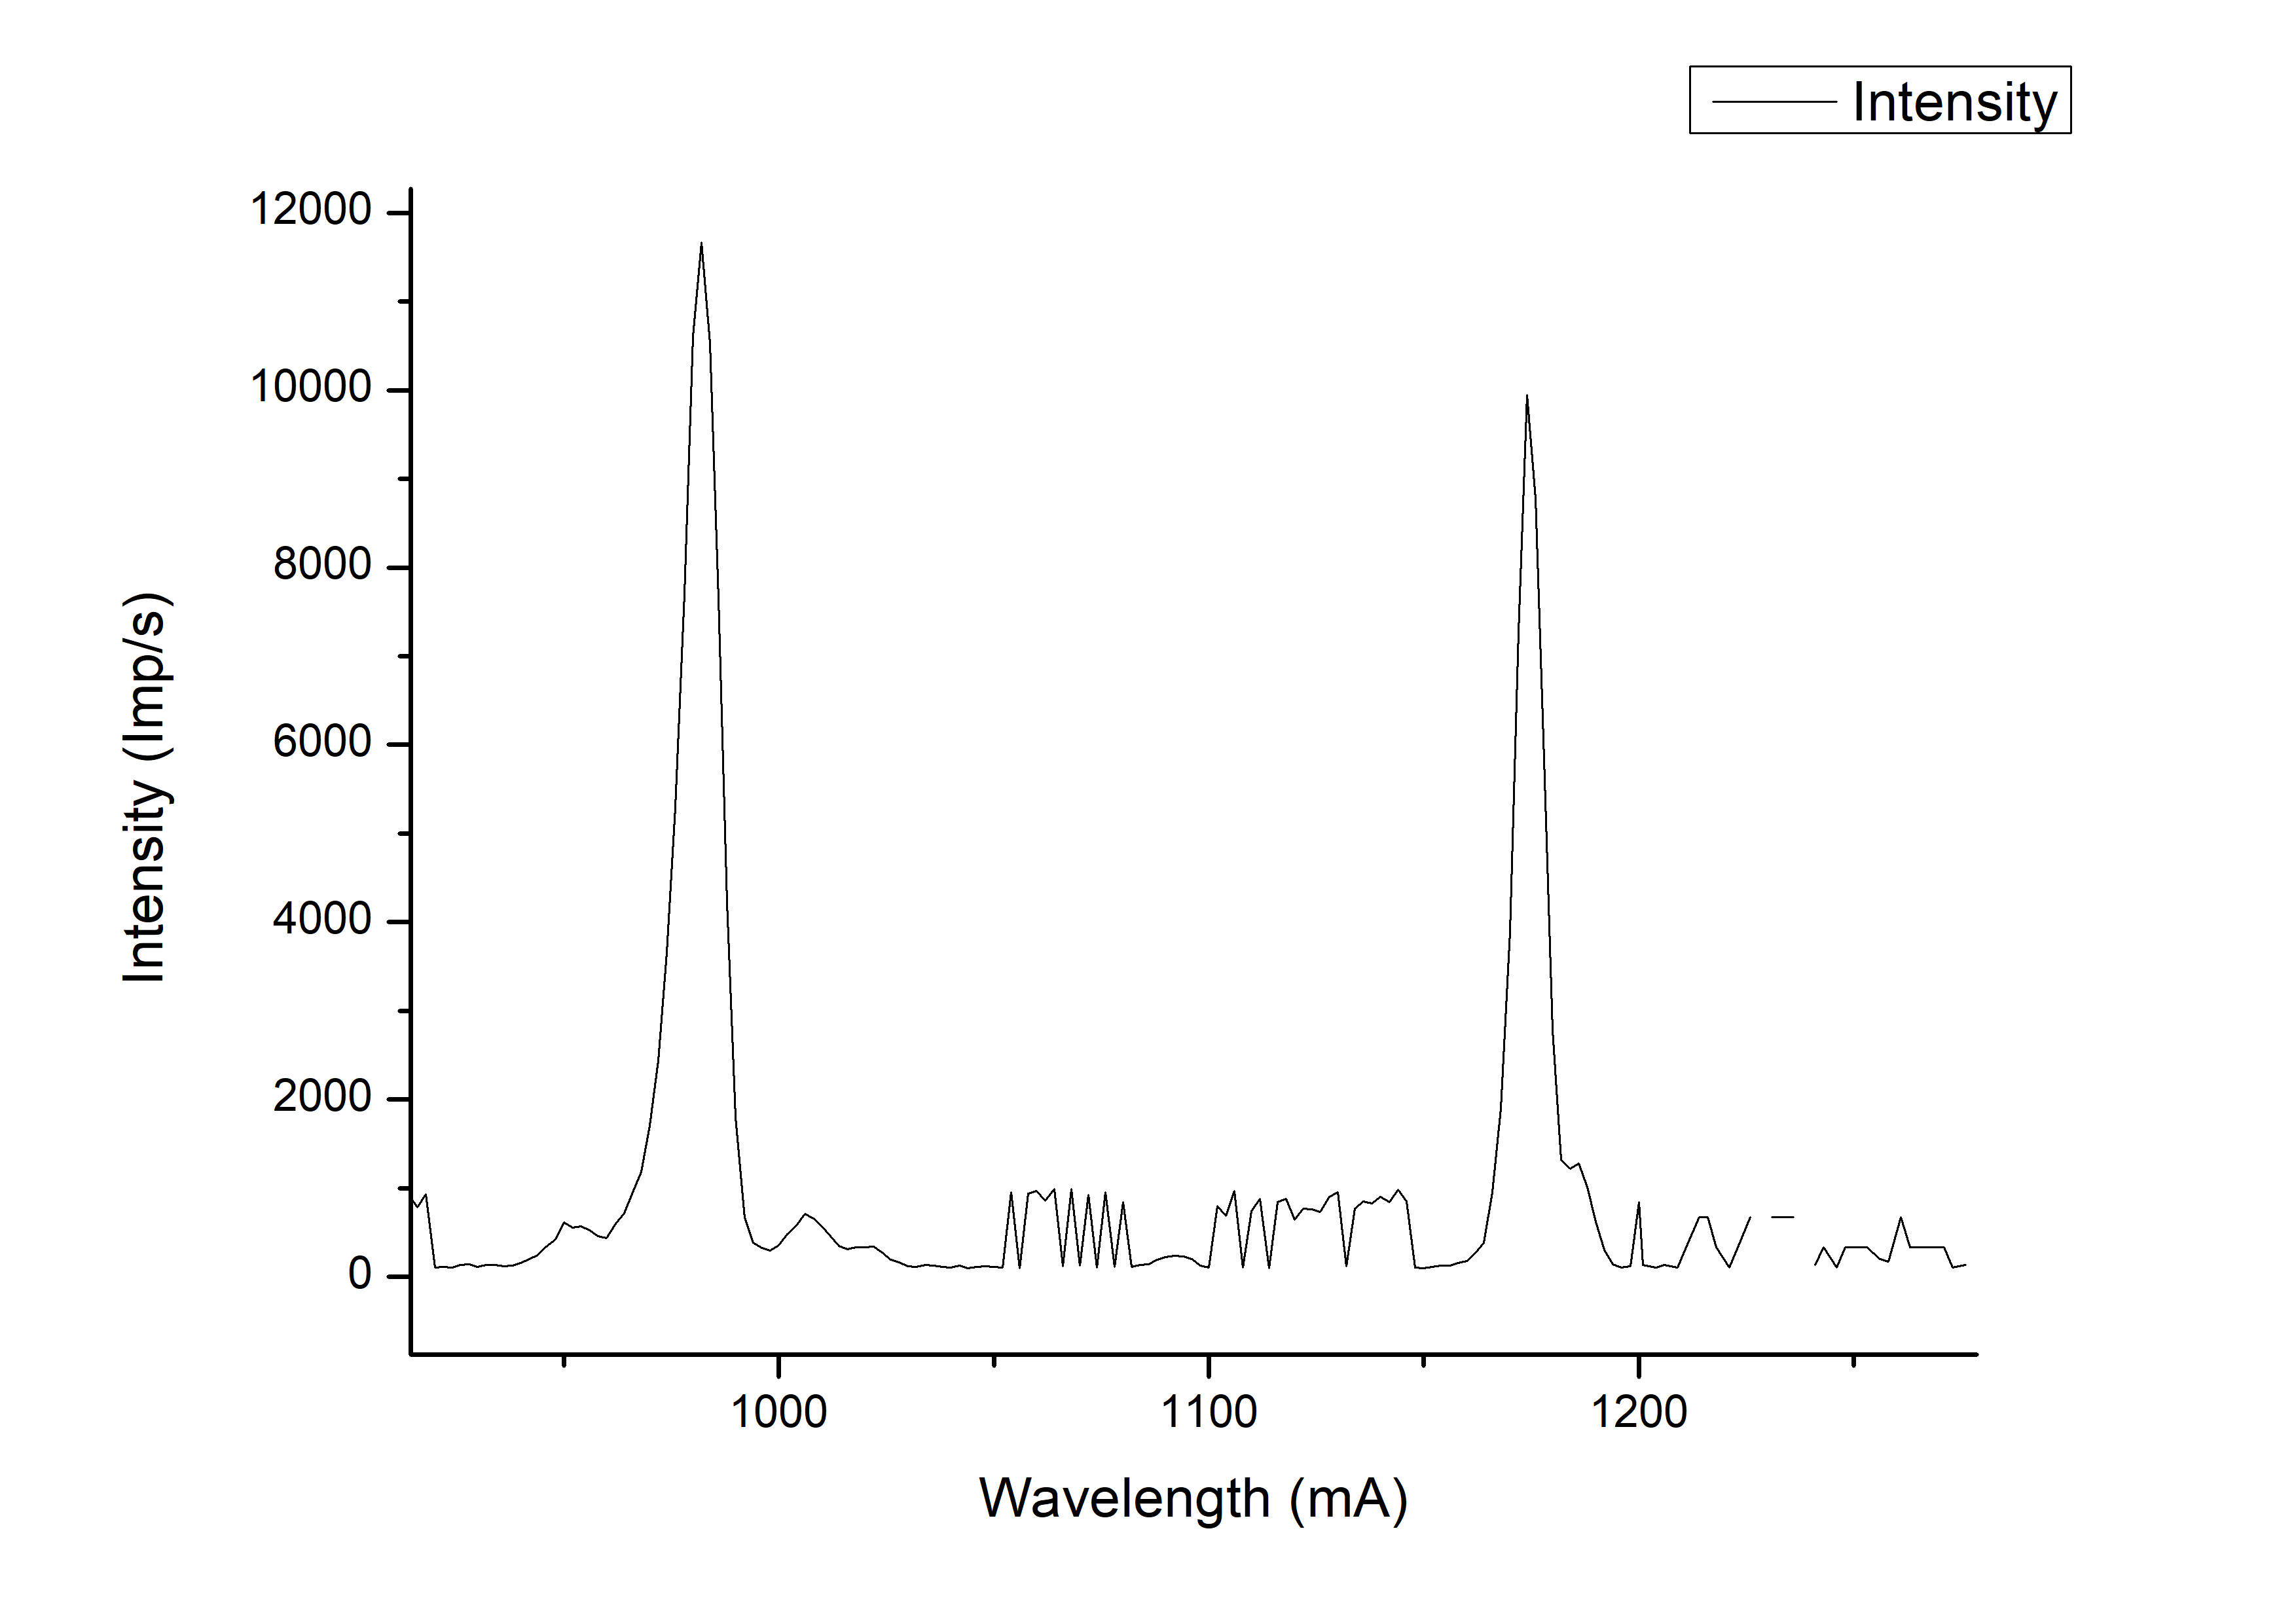
\includegraphics[width=1\linewidth]{Pb.png}
\caption{Спектр характеристического излучения свинца $^{82}$Pb} %% подпись к рисунку\label{ris:experimoriginal} %% метка рисунка для ссылки на него
\end{minipage}
\hfill 
\begin{minipage}[h]{0.45\linewidth}
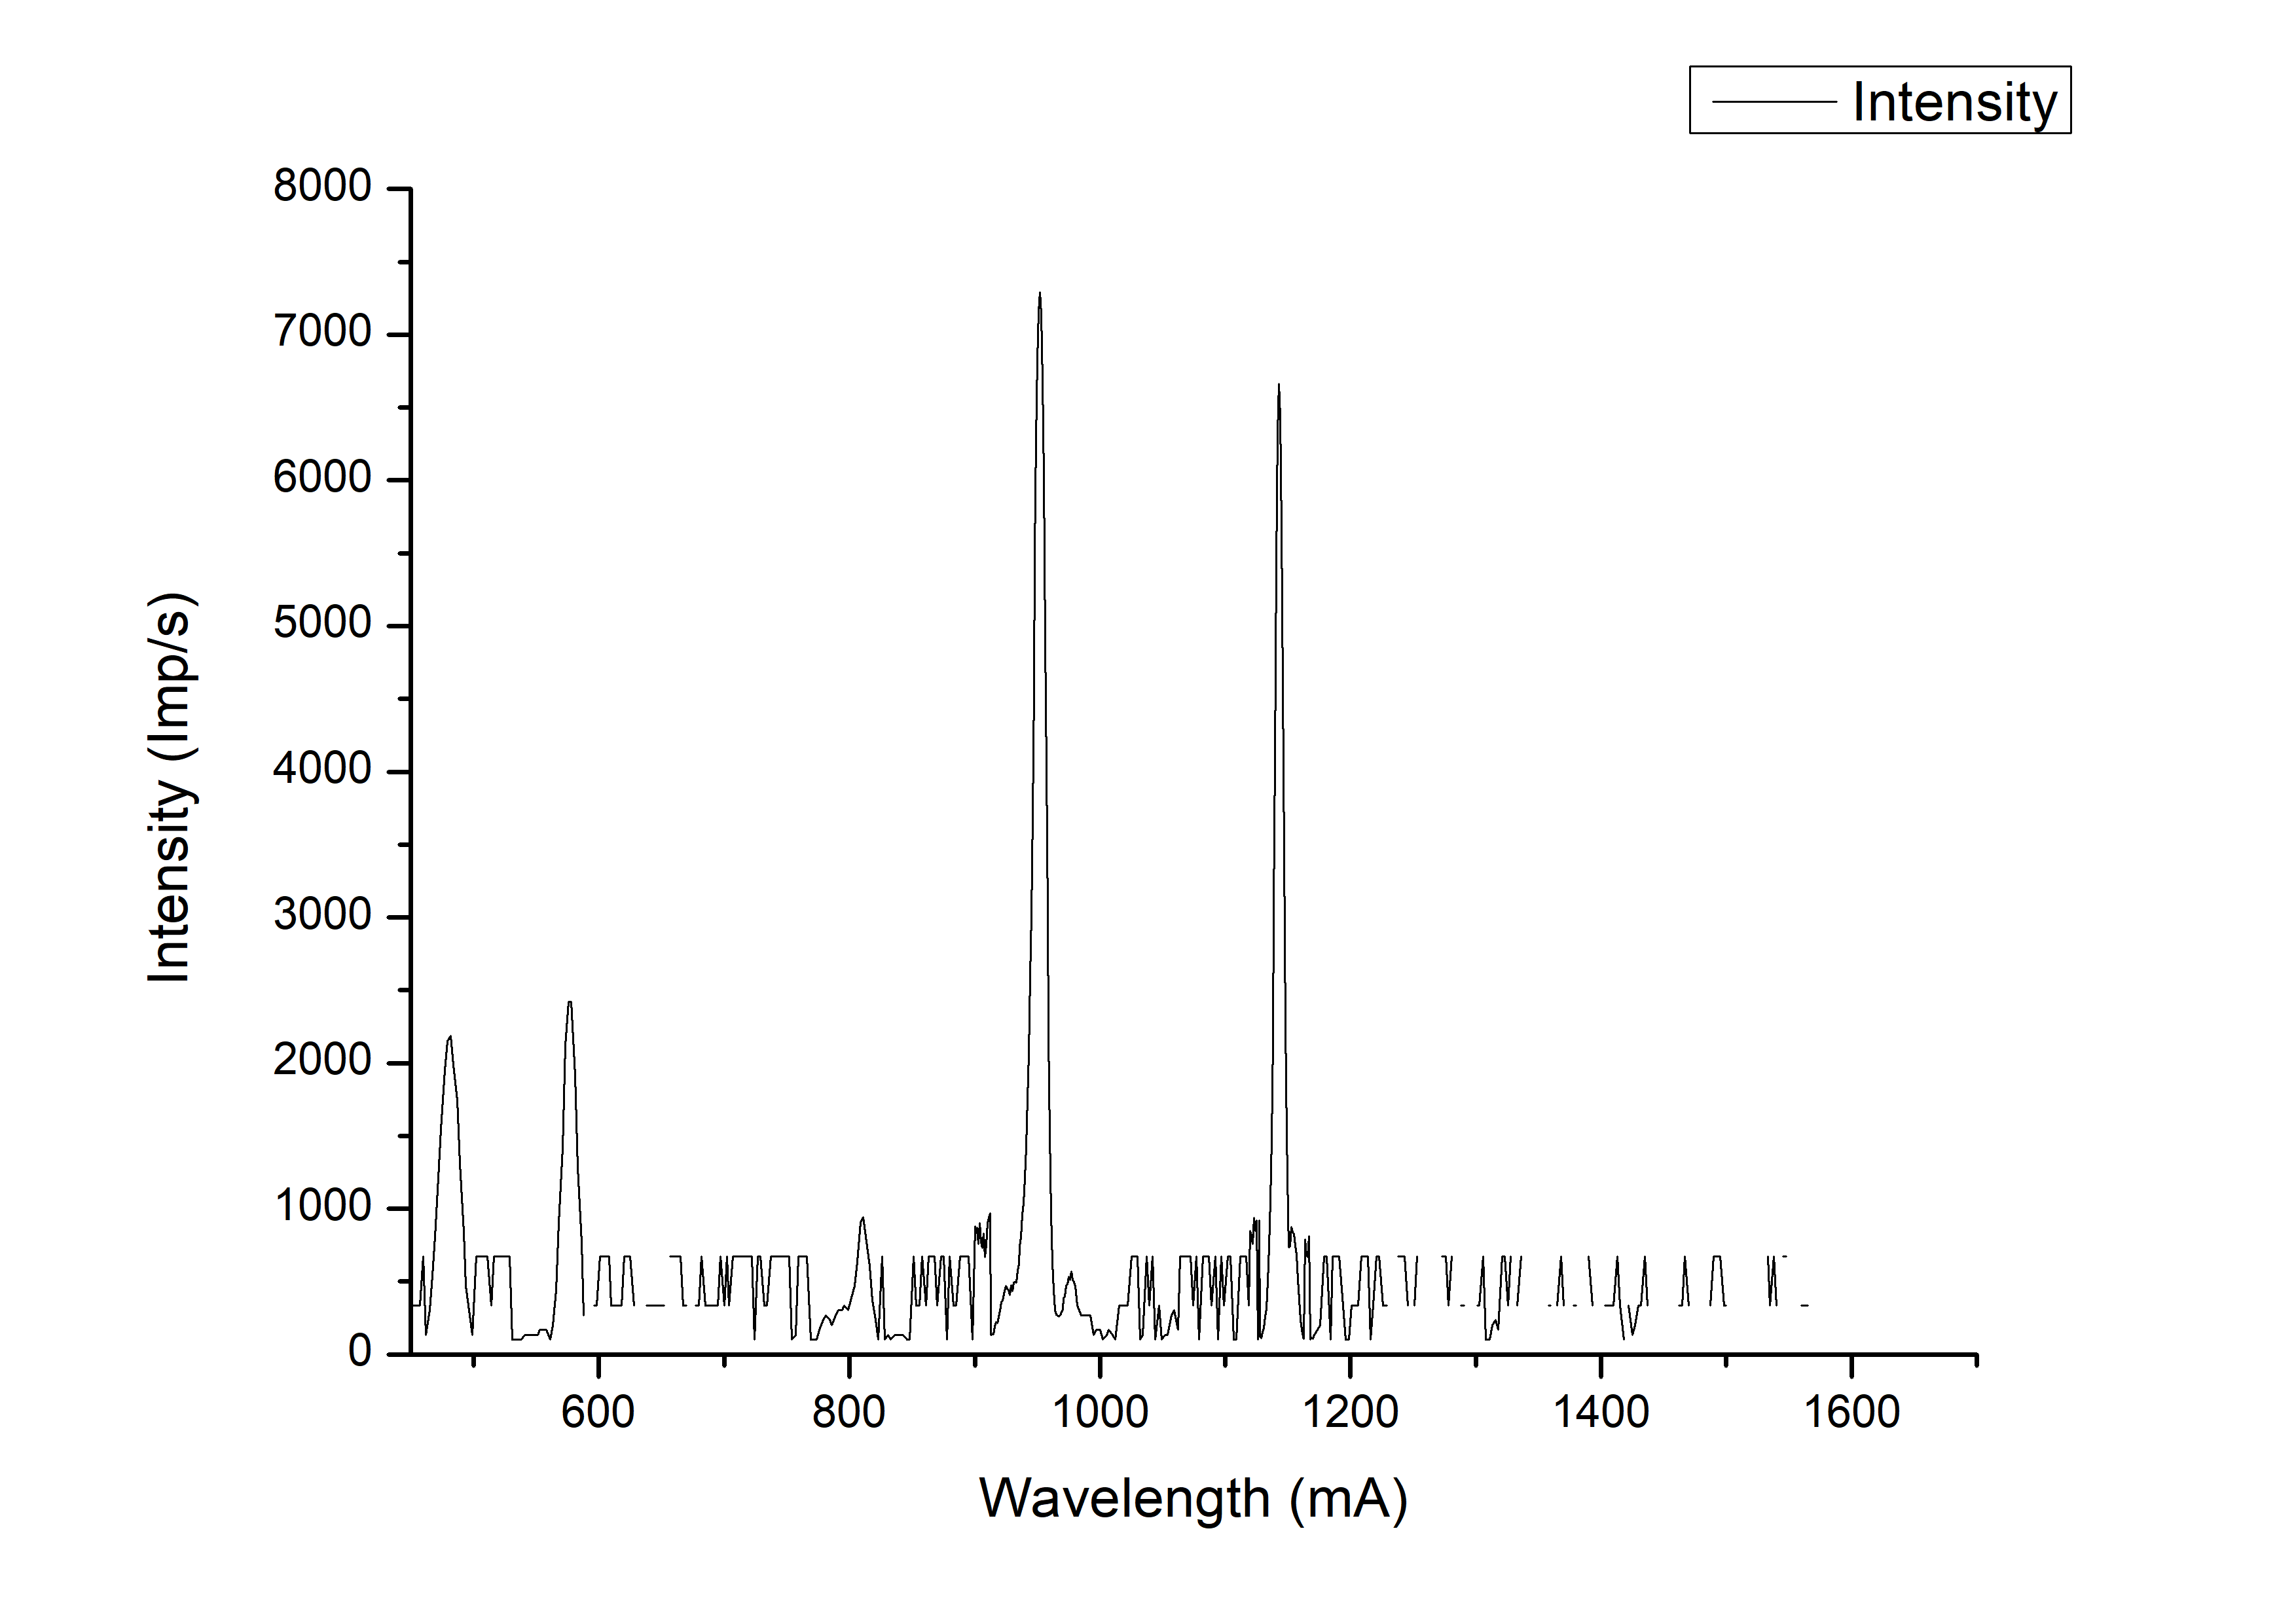
\includegraphics[width=1\linewidth]{Bi.png}
\caption{Спектр характеристического излучения висмута $^{83}$Bi}
\label{ris:experimcoded}
\end{minipage}
\end{center}
\end{figure}

\clearpage

\item Энергии соответствующих переходов определим по формуле $E = \frac{h c}{\lambda}$ (переведя в эВ из эрг). Также определим значения $\sqrt{\frac{E_{K}}{R_y}}$. Все значения занесём в таблицу 1.


    \begin{table}[h]
    \centering
    \begin{center}
    \caption{Анализ характеристического излучения различных элементов}
    \end{center}
    \vspace{0.1cm}
    \label{tab:my_label}
    \begin{tabular}{|p{1cm}|p{1cm}|p{2cm}|p{2cm}|p{2cm}|p{2cm}|p{2cm}|p{2cm}|}
\hline
 & $Z$ & $\lambda_{K_{\alpha}}$, m\AA & $\lambda_{K_{\beta}}$, m\AA & $E_{K_{\alpha}}$, эВ & $E_{K_{\beta}}$, эВ & $\sqrt{\frac{E_{K_{\alpha}}}{R_y}}$ & $\sqrt{\frac{E_{K_{\beta}}}{R_y}}$  \\
 \hline
Nd & 60 & 2369 & 2165 & 5247,5 & 5741,9 & 19,76 & 20,67
\\
 \hline
Tm & 69 & 1724 & 1528 & 7210,7 & 8135,6 & 23,17 & 24,61
\\
\hline
Yb & 70 & 1669 & 1473 & 7448,3 & 8439,4 & 23,55 & 25,06
\\
\hline
Lu & 71 & 1617 & 1421 & 7687,8 & 8748,2 & 23,92 & 25,52
\\
\hline
Ta & 73 & 1518 & 1317 & 8189,2 & 9439,1 & 24,69 & 26,51
\\
\hline
W & 74 & 1475 & 1281 & 8428,0 & 9704,3 & 25,05 & 26,88
\\
\hline
Pt & 78 & 1311 & 1119 & 9482,3 & 11109 & 26,57 & 28,76
\\
\hline
Au & 79 & 1275 & 1083 & 9750,0 & 11479 & 26,94 & 29,23
\\
\hline
Pb & 82 & 1174 & 982 & 10589 & 12659 & 28,07 & 30,70
\\
\hline
Bi & 83 & 1143 & 951 & 10876 & 13072 & 28,45 & 31,19
\\
\hline
\end{tabular}
\end{table} 

\item Построим график зависимости $\sqrt{\frac{E_{K}}{R_y}}$ от атомного номера $Z$ (рис. 13) и проверим выполнение закона Мозли

\begin{figure}[h]
\begin{center}
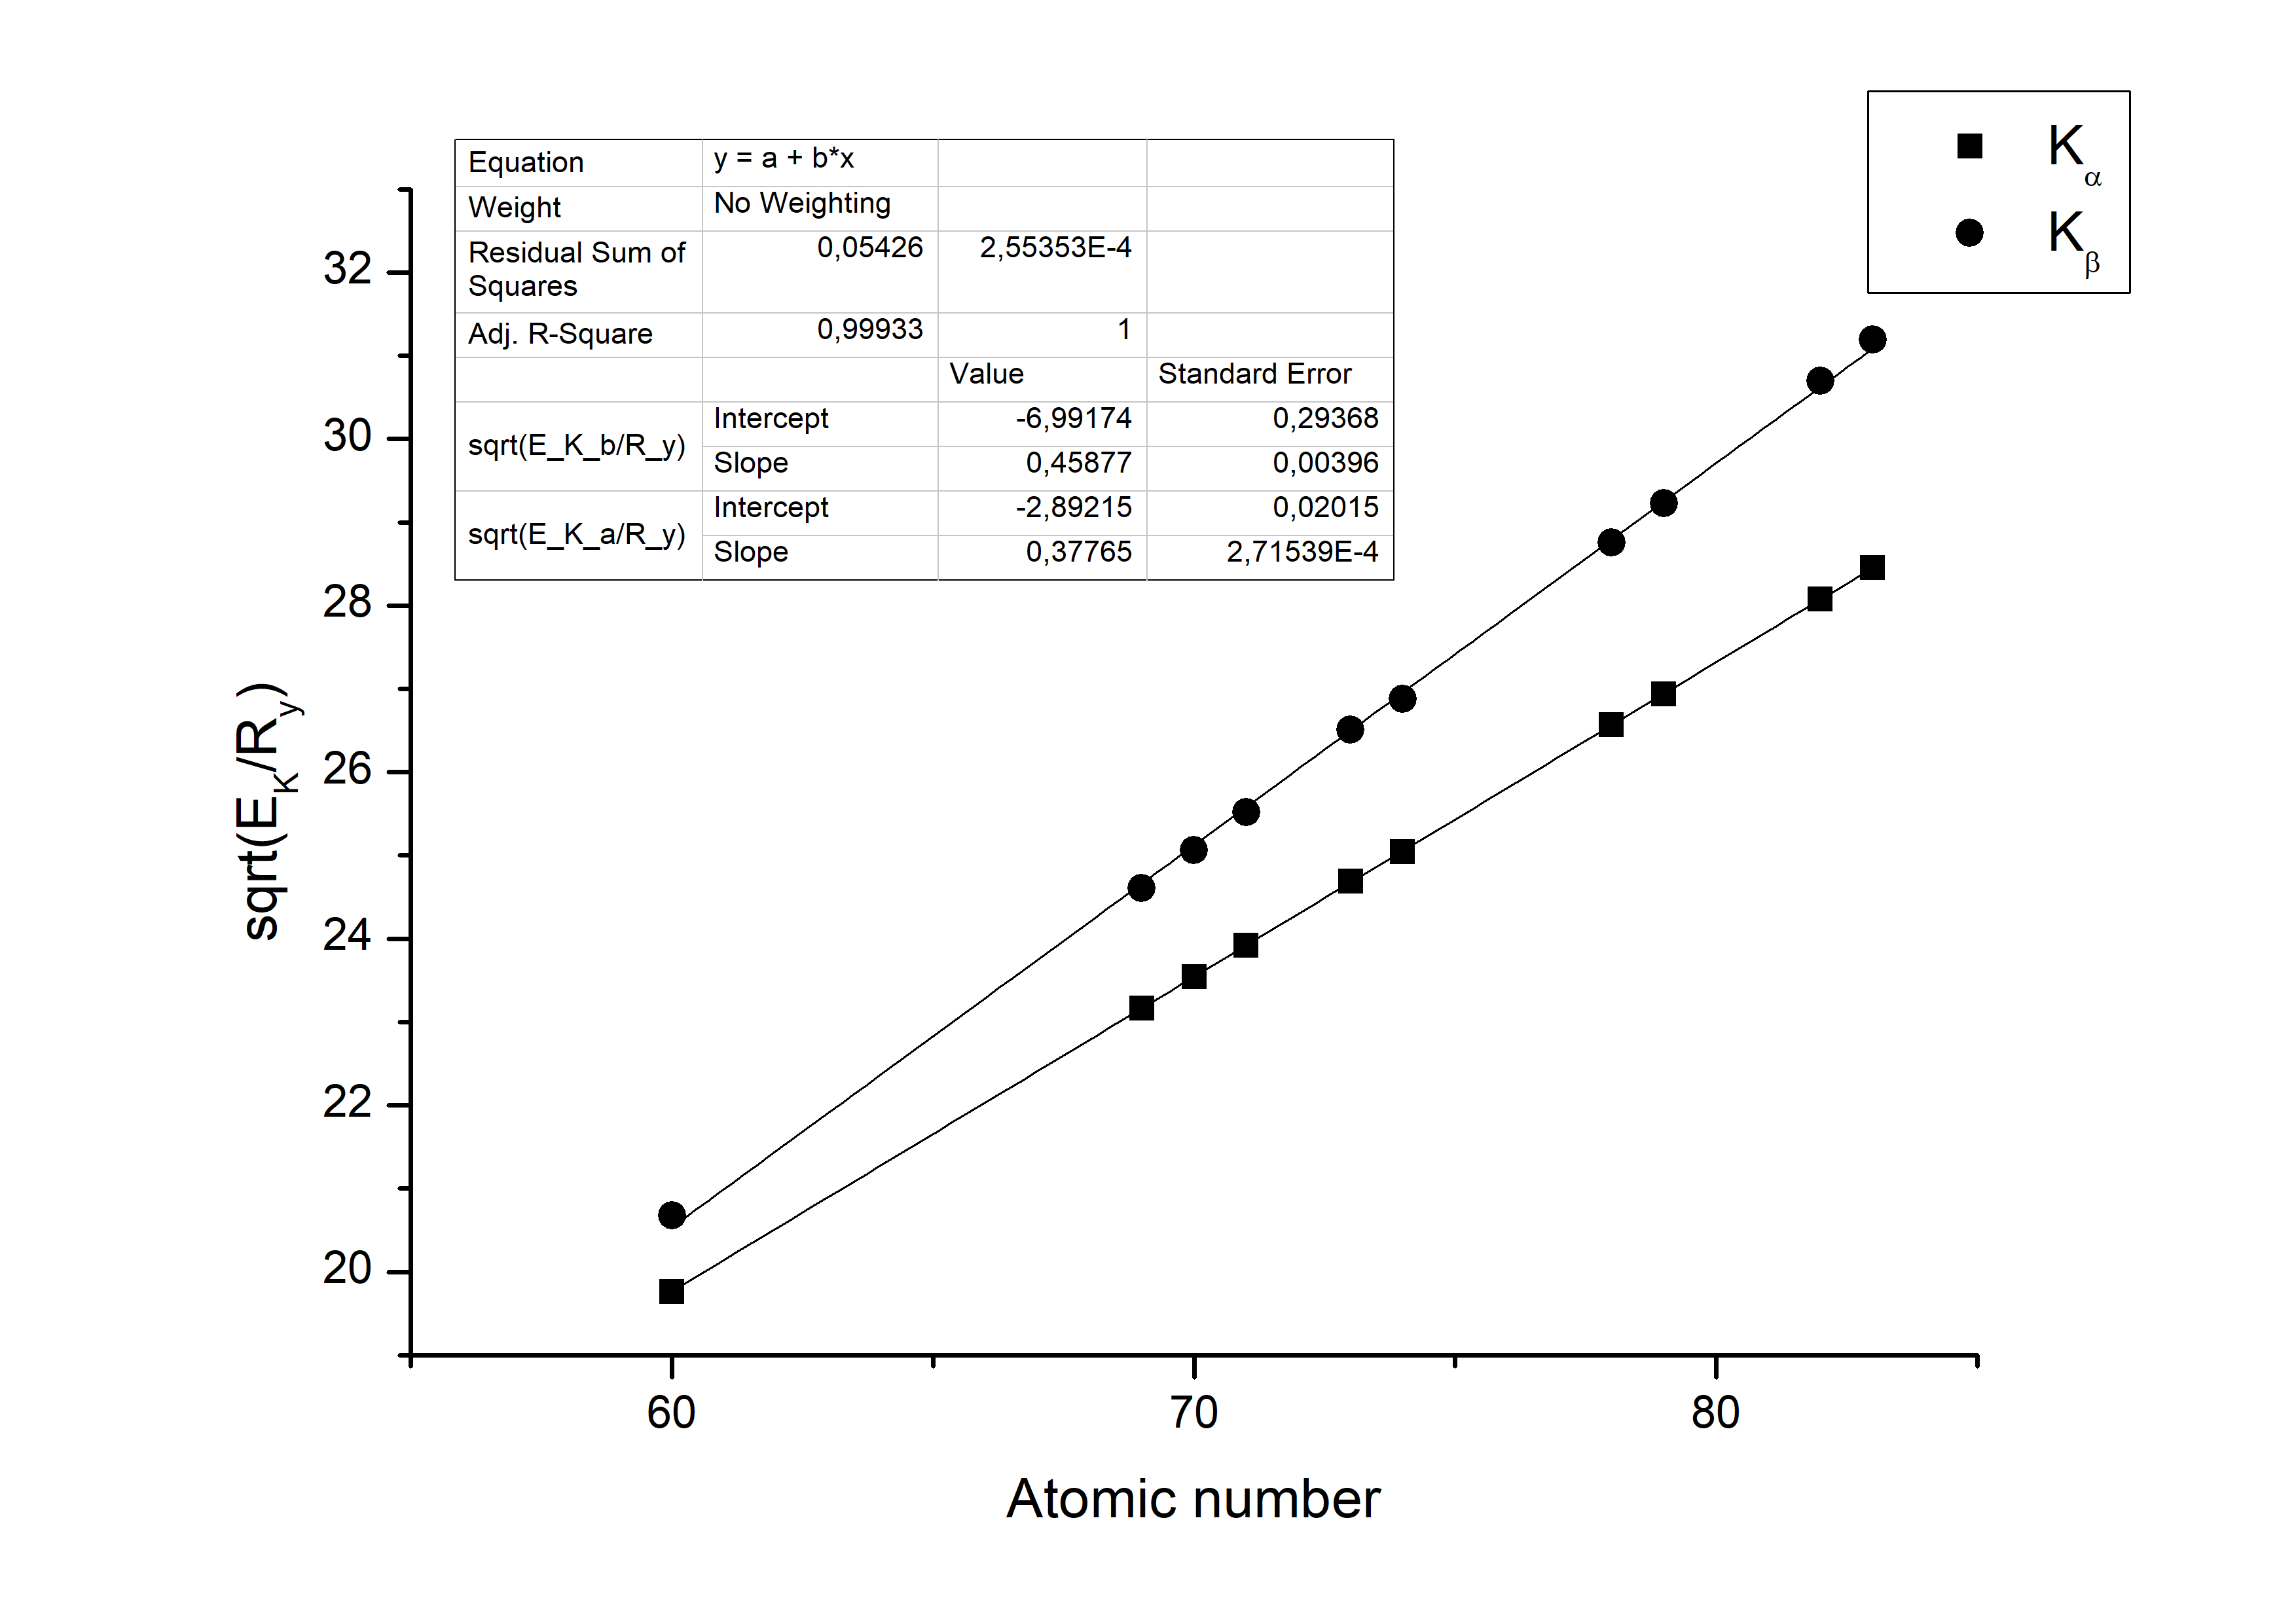
\includegraphics[width=15cm]{K_graph.png}
\caption{График зависимости $\sqrt{\frac{E_K}{R_y}}$ от $Z$}
\label{ris:experimoriginal} %% метка рисунка для ссылки на него
\end{center}
\end{figure}

\item Используя формулу (3) и полученные графики зависимости, определим постоянные $\sigma$ и $(\frac{1}{n_1^2}-\frac{1}{n_2^2})$

\begin{center}
    $\sqrt{\frac{E}{R_y}} = (Z - \sigma)\sqrt{(\frac{1}{n_1^2}-\frac{1}{n_2^2})} = Z\sqrt{(\frac{1}{n_1^2}-\frac{1}{n_2^2})} - \sigma \sqrt{(\frac{1}{n_1^2}-\frac{1}{n_2^2})} = Zb + a$  \\
    $b = \sqrt{(\frac{1}{n_1^2}-\frac{1}{n_2^2})}$ \\
    $\sigma = - \frac{a}{b}$
\end{center}

Тогда для наших коэффициентов:
\begin{center}
    $b_{L_{\alpha}} = 0,378$ \hspace{1cm} $b_{L_{\beta}} = 0,459$ \\
    $\sigma_{L_{\alpha}} = 7.65$ \hspace{1cm} $\sigma_{L_{\beta}} = 15.266$
\end{center}

Значения $b$  совпадают с теоретическими:
\begin{center}
     $b = \sqrt{(\frac{1}{n_1^2}-\frac{1}{n_2^2})}$ \\
     $L_{\alpha}: n_1 = 2, n_2 = 3$ \hspace{1cm} $L_{\beta}: n_1 = 2, n_2 = 4$ \\
     $b_{\alpha} = 0,373$ \hspace{1cm} $b_{\beta} = 0,433$ \\
\end{center}

\item В спектре контрольных образцов обнаружились следующие металлы:
\begin{itemize}
    \item золотая цепочка: золото, медь
    \item монета: цинк, медь
\end{itemize}

\end{enumerate}

\section{Вывод}

В ходе работы был изучен принцип работы рентгеновского спектрографа, измерены спектры характеристического излучения для ряда химических элементов. С помощью программного обеспечения были определены рентгеновские термы измеренных спектральных пиков излучения ($L_{\alpha}, L_{\beta}$). Построив зависимость $\sqrt{\frac{E_K}{R_y}}$ от $Z$ в ходе работы мы проверили справедливость выполнения закона Мозли (характер зависимости - квадратичный). \par
Были экспериментально определены коэффициенты экранировки для $L_{\alpha}, L_{\beta}$, а также значения $(\frac{1}{n_1^2}-\frac{1}{n_2^2})$, полученные значения с хорошей точностью совпадают с теоретическими (для серии $L_{\alpha}$ константа экранирования принимается равной 7,4)

\end{document}
